%************************************************
\chapter{Patterns of sitewise selection in mammalian genomes}
\label{ch_mammals1}
\acresetall
%************************************************

\section{Introduction}

This chapter describes the use of sitewise evolutionary estimates to
characterize the global distribution of selective constraint across 38
mammalian genomes and within the major mammalian superorders. I will
apply the Sitewise Likelihood Ratio Test, evaluated in Chapter
\ref{ch_indels1}, to the set of mammalian orthologous gene trees from
Chapter \ref{ch_orthologs} to generate genome-wide sets of sitewise
statistics measuring selective constraint in several groups of \mammln
species. Both this chapter and the following one are concerned with
the analysis of these data: here I will consider the overall
distribution of constraint observed in each set of genomes, while
Chapter \ref{ch_mammals2} will look at the application of \sw data to
identify gene- and domain-centric evolutionary trends.

I will first introduce the scientific context of this
project---namely, the sequencing and analysis of several mammalian
genomes for the \ac{mgp}---and outline the main questions motivating
the analysis I performed.

The next section will describe the preparation and alignment of the
mammalian gene tree from Chapter \ref{ch_orthologs} and introduce a
protocol for filtering genome-wide sitewise estimates. Although the
simulation study I performed in Chapter \ref{ch_indels1} showed that
sequences with divergence levels above that of most mammalian proteins
can be aligned without introducing many false positives due to
misaligning biological insertions and deletions, the analysis of
empirical sequence data involves many potential non-evolutionary
sources of alignment error. A sequenced and annotated genome is not a
piece of observed data; rather, it is the result of a succession of
inferences (based ultimately on the observation of a pool of genomic
DNA by some sequencing technology), each step along the way involving
potential errors and biases. Chapter \ref{ch_orthologs} looked at the
identification of mammalian orthologs, showing that the inference of
correct gene tree structures is fraught with difficulty and that \lcv
genomes are under-represented in gene duplications. Other sources of
error, including those occurring while reading DNA bases \citep{TODO},
assembling genomic fragments \citep{TODO}, and annotating gene-coding
regions \citep{TODO} have all been previously highlighted as being
important in the large-scale analysis of genomic data. As such, care
was taken to design and evaluate a variety of filters to reduce the
probability of yielding misleading results.

The third part of this chapter characterizes the global distribution
of mammalian selective constraint in three ways: first, using the \slr
statistic to identify sites evolving under purifying and positive
selection at various confidence levels; second, fitting parametric
distributions to the set of sitewise estimates to infer the
distribution of selective pressures; and third, evaluating the impact
of genomic variation in GC content and recombination rate on the
distribution of sitewise estimates.

\subsection{The Mammalian Genome Project}

A major goal of mammalian comparative genomics has been to quantify,
identify and understand the fraction of the human genome that is under
evolutionary constraint. The first non-human mammalian genomes showed
at least 5\% of the human genome to be under purifying selection
\citep{Mouse2002Initial,Rat2004Genome,LindbladToh2005Genome}, but the
small number of genomes available limited the extent to which regions
of evolutionary constraint could be identified. The \mgp, a
coordinated set of genome sequencing projects initiated in 2005 and
organised by the Broad Institute of MIT and Harvard, was designed with
the primary purpose of increasing the accuracy and confidence with
which regions of the human genome that have evolved under evolutionary
constraint in mammals could be identified \citep{Margulies2007}. In
line with this goal, 20 mammalian species were chosen for sequencing
in order to maximise the amount of evolutionary divergence available
for comparative analysis when combined with the 9 already available
sequenced genomes \citep{Margulies2005Initial}. Most of the 20
additional species were only sequenced to a target twofold coverage,
meaning each genomic base pair would be covered on average by two
sequence reads and roughly 85\% of genomic sequence would be covered
by at least one read. The decision to sequence many genomes at low
coverage was a deliberate choice, designed to maximize the average
amount of branch length available for the identification of
constrained sequence \citep{Margulies2007}.

As the \mgp proceeded from its sequencing to analysis phase in late
2008, it was clear that the additional branch length afforded by the
29-species phylogeny would enable a number of evolutionary analyses
beyond the identification of constrained non-coding regions. These
included the evolutionary characterisation of gene promoters,
identification of exapted non-coding elements, detection of
evolutionary acceleration and deceleration in non-coding regions, and
detection of purifying and positive selection in protein-coding
genes. Given the prior involvement of the Goldman group in analysing
the ENCODE comparative sequencing data
\citep{Margulies2007,ENCODE_Project_Consortium2007a} and Tim
Massingham's development of the SLR software for sitewise evolutionary
analysis \citep{Massingham2005}, the group was recruited to perform
the protein-coding evolutionary analysis for the \mgp, and the project
turned into a portion of my PhD research. This chapter describes my
work on the project, which began in late 2008; all of the work
described below was performed by me, though I benefitted greatly from
advice and discussion with members of the Goldman group (Nick Goldman
and Tim Massingham), the EnsEMBL Compara team (Albert Vilella, Javier
Herrero, Ewan Birney) and the organisers and members of the \mgp
(especially Manolis Kellis, Kerstin Lindblad-Toh, Mike Lin, and, Katie
Pollard). The major results from the initial version of this analysis
have recently been published \citep{LindbladToh2011}; the work
presented below includes some improvements to the filtering and
alignment methodology and incorporates sequence data from a number of
genomes which were restricted from use in the \mgp analysis.

\section{Data quality concerns: Sequencing and assembly error in evolutionary analysis}

The possibility that erroneously-aligned sequences might cause false
positives in the detection of sitewise positive selection was a major
concern for this analysis, especially given the \lcv nature of the 20
newly-sequenced genomes. Although the \slr test and other \sw \ml
methods have been shown to be conservative in their identification of
positively selected sites under most conditions, even when the amount
of data is low or the null model is violated
\citep{Anisimova2002,Anisimova2003,Massingham2005}, most evolutionary
analyses are based on the assumption that all sites within an
alignment column are truly homologous. This assumption can be violated
in a number of ways, some of which are described below.

Of course, alignment error can result from errors in reconstructing
the evolutionary history of sequences evolving with indels, causing
non-homologous codons to be placed in the same alignment column. In
Chapter \ref{ch_indels1} I explored the tendency of a number of
progressive multiple alignment programs to produce such errors,
showing that \prankc alignments introduce few falsely identified
positively-selected sites resulting from alignment errors at
mammalian-like divergence levels. Thus, \prankc was used to align all
coding sequences, and the number of false positives resulting from
misalignment of biological insertions and deletions was expected to be
low.

However, biological indels are not the only potential source of
misalignment error. Errors resulting from the inclusion of incorrect
genomic sequence in coding sequences were an additional
concern. Twenty of the genomes under study were sequenced at low
coverage and were not assembled into chromosomes or finished to
completion, making the likelihood of miscalled bases, spurious
insertions or deletions, or shuffled regions due to mis-assembly
relatively high \citep{Green2007}. The magnitude of the effect of each
of the aforementioned types of sequence errors on the detection of
positive or purifying selection depends on the nature of the inference
method, the type of sequencing error, and the branch length of the
terminal lineage leading to the species containing the sequence error.

As most codon-based inference methods assume independence between
amino acid sites, the effect of misalignment on the resulting
inference will be independent between neighboring codons. Thus, one
may first consider the effect---in isolation---of a single
spuriously-assigned homologous codon on the \ml estimation of
\omg. Two distinct situations can be encountered: first, the case
where a single sequence error causes one spurious nucleotide
substitution within a codon, and second, the case where one or
multiple sequence or assembly errors cause multiple spurious
substitutions within a codon. Single spurious nucleotides, such as
miscalled bases, would add noise to the estimation of \omg, but as a
whole they would not be expected to cause false positive positively
selected codons. If we assume no large difference between the natural
mutational process and the process that caused the erroneous mutation
(e.g., a random distribution across codon positions and no bias in the
identity of the miscalled base) then the effect would be to shift the
estimated \omg in the branch containing the error towards 1. This is
because, on average, isolated miscalled bases would appear the same as
a neutral substitution process, inflating the estimated substitution
rate but not affecting the relative \nsyn and \syn rates.

In contrast to single spurious substitions, codons with multiple
erroneous bases in one species may produce strongly elevated inferred
substitution rates and \omg estimates. This is due to the necessity of
the codon model implemented in SLR to infer a multi-step path of
single substitutions between the two codons on either side of a given
evolutionary branch. The exact \ml path estimated between two
completely non-homologous codons depends on the estimated codon
frequencies, the branch length separating the two sequences, and the
nature of the process causing misalignment of nonhomologous codons,
but in general it would be reasonable to expect a greater number of
false positive \pss{}s resulting from codons with multiple erroneous
bases than from codons with single errors due to the necessary
inference of a multi-step path between codons with multiple nucleotide
differences.

Given the potentially greater impact of codons with multiple errors,
the propensity of each of the common sequencing error types identified
above (miscalled bases, spurious indels, and
shuffled/repeated/collapsed regions due to mis-assembly) to cause
single or multiple errors within codons could strongly affect its
impact on the sitewise detection of positive selection. On its own, a
miscalled nucleotide base would obviously result in a single spurious
substitution. However, low-quality bases tend not to be uniformly
distributed among or within sequence reads \citep{Kircher2009},
increasing the probability of multiple errors within a codon resulting
from miscalled bases. Spurious indels within coding regions may be
even more likely than miscalled bases to cause multiple errors within
a codon due to the potential for creating frameshift
artifacts. Assembly errors, which result in larger-scale structural
errors including missing, repeated, shuffled or inverted sequence
regions \citep{Jaffe2003}, are especially prone to producing codons
with multiple erroneous substitutions due to the large amount of
contiguous sequence data being misplaced.

For detecting positive selection, the nature of the model used for
inferring positive selection and the branch lengths separating the
species being tested may also have an impact on the prevalence false
positives resulting from sequence errors. Sequence errors should only
substantially affect the estimation of \nsyn and \syn substitution
rates along the terminal lineage leading to the erroneous sequence
data; thus, the potential impact of sequencing error on the inference
of a positively selected site or gene can be estimated by considering
the potential impact of an inflated rate of \nsyn substitution along
the terminal branch on the inference of positive selection with a
given test. Both the branch-site test for positive selection (which is
not used in this analysis) and the sitewise tests for positive
selection (including \pamlEight and \slr, first described in Chapter
\ref{ch_indels1}) are sensitive to erroneous substitutions occurring
at individual alignment columns, with the major difference between the
two types of test being that the branch-site test is highly sensitive
to substitutions along the foreground branch(es) being tested for
positive selection, while sitewise tests only measure the signal for
positive selection across the entire evolutionary tree.

For the branch-site test, the potential effect of sequencing error
should depend on the location and length of the foreground branch(es):
if the terminal branch leading to the spurious sequence is within the
foreground, and especially if it represents a sizeable portion of the
overall foreground branch length, then false positives could easily
result; if, however, the terminal branch is outside of the foreground,
then it would have little direct impact on the \fpr of the branch-site
test aside from adding noise to the estimation of parameters in the
non-foreground branches of the tree.

For site-based tests such as \slr, the effect of sequencing error
should be independent of the position of the terminal branch within
the tree, depending more on the magnitude of \nsyn substitution rate
elevation resulting from the sequence error and the fraction of total
branch length covered by the ``erroneous'' terminal branch within the
phylogenetic tree being studied. It would be difficult to consider
each of these factors (the terminal branch length and the magnitude of
\nsyn substitution rate elevation) in isolation due to their
non-independence: sequence errors in a short terminal branch may yield
a strongly elevated \nsyn substitution rate, but the impact on the
overall inference of positive selection may be limited as a result of
the short branch length. On the other hand, the same erroneous
sequence in a species with a longer terminal branch would likely cause
a smaller elevation in the \nsyn substitution rate (due to the higher
expected number of substitutions along a longer branch) yet the impact
of such an elevated rate on the sitewise inference would be
proportionally greater due to the higher branch length. A reasonable
hypothesis would be that these opposing factors would effectively
cancel each other out in the \ml calculations. In either case, the
expectation that a phylogeny with a greater proportion of its branch
length within terminal branches (which, in contrast to internal
branches, may contain spurious substitutions resulting from sequencing
errors) would be more prone to false positives should still hold.

To summarize, the expected effect of alignment errors on the sitewise
detection of positive selection should be minimal when using a good
aligner and analysing data within vertebrate divergence levels, but
the number of false positives resulting from sequence errors depends
on a number of factors including the frequency, spatial clustering,
and terminal branch length associated with sequencing, assembly and
annotation errors. In some cases, even a relatively large amount of
sequencing error may not produce a strongly elevated \fpr (e.g., when
the total internal branch length is large as when analyzing all
mammals or vertebrates), as the addition of a few spurious
substitutions would not significantly change the estimated \nsyn
substitution rate. In other cases, however (e.g., when teh branch
length is small, and/or many low-quality genomes are included), it may
significantly bias results towards excess false positives.

\subsection{Empirical studies of the influence of sequencing and annotation errors on detecting positive selection}

Simulation studies similar to those I performed in Chapters
\ref{ch_indels1} and \ref{ch_indels2} could improve our understanding
of the relative potential of different types of sequencing errors to
introduce false positives in downstream analyses, but the absolute
frequency and pattern of such errors would still difficult to predict
without a reliable model for their generation. This is especially true
for larger-scale errors from misassembly or misannotation, which are
less easily modeled than base calling errors and could have
potentially more significant negative effects. Thus, for estimates of
false positives resulting from these types of sequence errors, an
empirical approach seems more appropriate. In particular, two
empirical studies in mammals have provided convincing evidence that
sequence, alignment and annotation errors can drastically increase the
number of false positive \psg{}s in the branch-site test for positive
selection.

Schneider et al. \citeyearpar{Schneider2009} performed a genome-wide
scan for positive selection in the terminal branches of 7 mammalian
genomes using the branch-site test and analysed the fraction of
\psg{}s within subsets of high- or low-quality genes according to
three sequence and alignment quality metrics. They found that the
fraction of \psg{}s was significnatly higher for genes exhibiting
lower quality sequence, annotation and alignment metric, with genes in
the highest-quality and lowest-quality categories showing a 7.2-fold
difference in the inferred fraction of \psg{}s
\citep{Schneider2009}. This observation provided evidence of a
correlation between the chosen quality metrics and the tendency of an
alignment to exhibit positive selection. It did not necessarily imply
causation, however, as the same result might have been observed---even
in the absence of sequence error---if some biological properties of
the true \psg{}s caused them to yield lower quality metrics than
non-\psg{}s. Looking at the three metrics used in their study
(sequencing coverage, gene annotation status, and alignment quality
according to the heads-or-tails method), it is plausible that
properties associated with elevated \omg ratios and positive
selection, such as recent gene duplication
\citep{Beisswanger2008,Studer2008,Casola2009}, high GC content
\citep{Ratnakumar2010} or functional shifts \citep{Storz2008,Wang2001}
might have had an error-independent effect resulting in a higher
proportion of \psg{}s in low-scoring categories. The heads-or-tails
method has also been shown to be inappropriate for estimating
alignment uncertainty \citep{Fletcher2010}, so results based on this
measurement should be taken with caution. Despite these criticisms,
the analysis did provide good evidence that some of the obvious
sources of error may be contributing to excessive estimates of
branch-specific positive selection in mammals.

Mallick et al. \citeyearpar{Mallick2009} took a different approach to
the same problem by performing a careful resequencing and reassembly
of the chimpanzee genome (the initial assembly of which had lower
coverage and lower quality than the human genome) and re-analysing the
evidence for positive selection along the chimpanzee linegae in 59
genes which had previously been identified as chimpanzee \psg{}s. The
authors, who were motivated by a concern that previous reports of a
larger proportion of \psg{}s in chimpanzee than in human
\citep{Bakewell2007} were the result of its lower-quality genome
rather than a biologically significant difference in levels of
adaptation, found that the vast majority of \psg{}s identified in two
previous studies showed no evidence for positive selection when using
their reassembled and higher-coverage version of the chimpanzee genome
\citep{Mallick2009}. This suggested that the original 4x coverage
chimpanzee genome contained a number of sequencing and assembly errors
leading to false inferences of positive selection. A detailed analysis
of 302 codons with multiple spurious \nsyn substitutions in the
original assembly showed roughly comparable effects of sequence error
(explaining 23\% of codons), assembly error (14\% of codons) and local
alignment error (30\% of codons).

Taken together, the results of Schneider et
al. \citeyearpar{Schneider2009} and Mallick et
al. \citeyearpar{Mallick2009} provide strong evidence in support of
the hypothesis that errors in sequencing, assembly, annotation and
alignment can result in strongly elevated inferred \omg values when
using sensitive tests for detecting positive selection. Furthermore,
the detailed identification and quantification of error sources
performed by Mallick et al. \citeyearpar{Mallick2009} provided an
empirical estimate of how important each potential source of error
would be in the detection of positive selection. Although both of
these studies used the branch-site test for detecting positive
selection, their results could be expected to generalize well enough
to guide the design of filtering methods for the present \sw
analysis. With this work in mind, I implemented three filtering steps
to help identify and remove sequences and alignment regions
potentially subject to the errors noted above: filtering out
low-quality sequence, removing gene fragments and recent paralogs, and
identifying alignment regions with excess clustered substitutions.

\subsection{Filtering out low-quality genome sequence}

Due to the presence of several low-coverage genome assemblies in the
set of available mammalian genomes and the elevated sequencing error
rates in such assemblies \citep{Hubbard2007}, I applied a conservative
filter to the set of input sequences based on sequence quality scores
where available.

Most automated genome assembly pipelines, such as the Arachne tool
used to sequence many of the low-coverage mammalian genomes
\citep{Jaffe2003}, output a set of Phred quality scores alongside the
identified genome sequence, with one Phred score per base ranging in
value from 0 to 50. A Phred score represents the probability,
calculated by the sequencing and/or assembly program, that a given
base call is incorrect. This probability is usually concisely
expressed as the negative logarithm of the probability of an error
multiplied by ten, or $Q=-10log_{10}P$, where $Q$ is the Phred score
and $P$ is the probability of an incorrect base call \citep{Cock2010}.

Although \ens was used as the source for gene sequences in this
analysis, it does not store quality scores from its source genome
assemblies, so Phred quality scores were manually downloaded for all
genomes with readily available Phred-like quality scores (see Table
\ref{table_phred} for the assembly versions and URLs from which
quality score files were downloaded). Most quality scores were
provided as a single file in FASTA format with one string of numerical
scores per assembled contig. Since the process of filtering a single
mammalian coding alignment required collecting scores from many
different quality score files for many disjoint genomic locations, a
custom script was written to process each quality score file to allow
for faster score retrieval and better memory performance. In total,
quality score files for XYZ genomes were indexed and used for quality
filtering.

A suitable score threshold for filtering coding regions was chosen
based on a study by Hubisz et al. \citeyearpar{Hubisz2011}, who
performed a detailed analysis of Phred quality scores, which are a
probabilistic prediction of the error rate, and actual error rates in
low-coverage mammalian genome assemblies by comparing the low-coverage
assemblies to matched regions of high-quality sequence from the ENCODE
comparative genomics dataset
\citep{ENCODE_Project_Consortium2007a}. The authors identified a
strong correlation between Phred scores and actual error rates for
scores below 25, indicating that the scores were accurate predictors
of the true error rate in this range. Error rates did not decrease
significantly at scores above 25, however, suggesting that the use of
an extremely high Phred score threshold would only minimally reduce
error levels below those obtained with a moderate
threshold. Furthermore, Hubisz et al. noted that 85\% of bases in the
low-coverage mammalian genomes contain very high Phred scores ($>45$)
and only 4\% have low scores ($<20$).

Based on these observations, a threshold Phred score of 25 was chosen
as a reasonable trade-off between the potential benefit of avoiding
miscalled bases and the potential cost of masking out correctly
sequenced bases. For each protein-coding sequence with quality scores
available, a ``minimum score'' approach was used to filter out whole
codons: all codons containing one or more nucleotides with a score
below 25 were masked out with three ambiguous nucleotides, 'NNN'.

The expected proportion of filtered nucleotides could be calculated
from the fraction of bases below the Phred score threshold of
25. According to Hubisz et al. \citeyearpar{Hubisz2011}, approximately
5\% of bases in low-coverage mammalian genomes contain Phred scores
below 25. The worst case scenario (e.g., the worst case in terms of
the number of high-quality bases being masked as a result of using the
minimum score approach) would be if only one base per codon had a
score below the threshold. In that case, an expected 15\% of
nucleotides would be filtered, since 3 bases would be masked for every
low-quality base. However, the distribution of low-quality bases is
likely highly clustered, due to the uneven distribution of
repetitiveness and GC content as well as the tendency for uncertain
base calls to occur towards the end of sequence reads (all of which
are known to affect read coverage and assembly performance,
e.g. \cite{Teytelman2009}). A more clustered distribution of
low-quality bases would cause fewer high-quality bases to become
masked by the minimum score approach, reaching the limit of an
expected 5\% total filtered bases if low-quality bases always occurred
in groups of three and were positioned along the boundary of codon
triplets. Thus, anywhere from 5\% to 15\% of nucleotides from
low-coverage genomes were expected to be filtered by this approach.

\begin{figure}
\centering
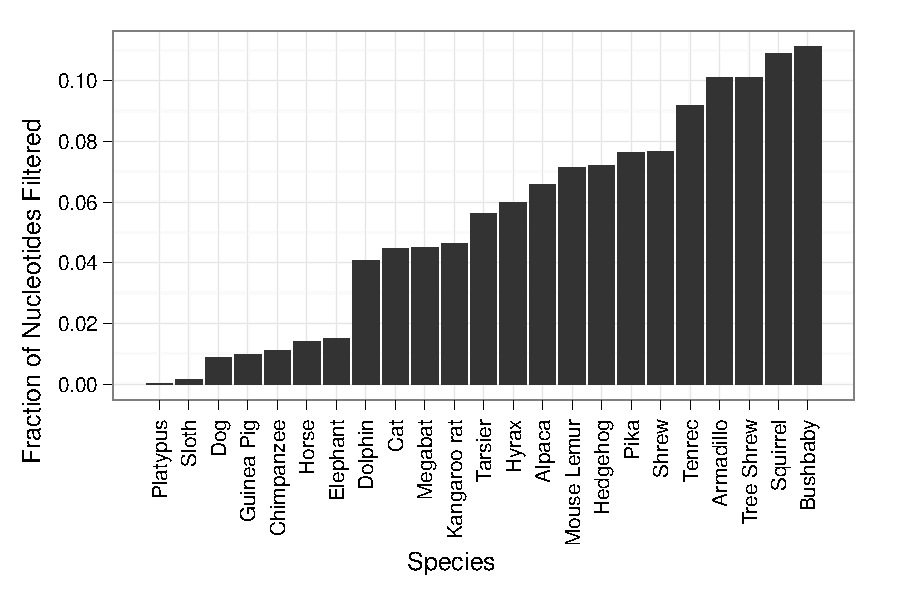
\includegraphics[scale=0.7]{Figs/filtered_qual_bars.pdf}
\caption{}
\label{filtered_qual_bars}
\end{figure}

The above filtering scheme was applied to all coding sequences from
each species for which quality scores were available, which included
all of the species with \lcv genomes as well as five with
high-coverage genomes: chimpanzee, guinea pig, dog, horse, cow, and
elephant. The overall percentage of nucleotides filtered from each
genome is shown in Figure \ref{filtered_qual_bars}. As expected,
genomes with high-coverage sequences contained fewer bases with low
Phred scores, resulting in 1-2\% of nucleotides being filtered. The
bulk of low-coverage genomes resulted in 4-8\% of nucleotides being
filtered, while five genomes (bushbaby, squirrel, tree shrew,
armadillo and tenrec) showed a noticeably higher proportion of
low-quality bases, with 9-11\% nucleotides being filtered out. The
distribution of filtered nucleotide proportions confirmed the
expectation that 5-15\% of nucleotides would be filtered using a Phred
score threshold of 25, and the variation in filtered nucleotide
proportions between different species showed that despite the uniform
2x coverage of the \lcv mammalian genomes, different assemblies varied
widely in their distributions of sequence quality scores within coding
regions. 

\subsection{Removing recent paralogs}
\label{section_removing_paralogs}

To complement the \subtr{} splitting process, which split apart
ancient duplications to avoid paralogous comparisons in the sitewise
analysis, a second paralog filtering step was implemented to result in
no more than one sequence per mammalian species existing in each gene
tree. Some of these apparent paralogs likely resulted from gene
duplications that occurred subsequent to the two rounds of
whole-genome duplication in the vertebrate ancestor, but it was also
expected that a sizeable proportion of apparent paralogs in the
Ensembl gene trees were the result of errors in gene annotation or in
the inference of gene trees by the \cmp pipeline.

A particular cause for concern in the current analysis was the
possibility that stretches of missing or unassembled sequence in \lcv
genomes might have produced gaps of missing data or assembly
breakpoints between exons of a single gene, causing it to become
annotated as two separate genes. These shortened genes would be
treated as independent proteins by the \cmp pipeline, likely being
placed at very similar positions in the gene tree due to each having
been derived from the same single source gene. While this result might
not be detrimental to sitewise analysis in itself (as each shortened
gene might be correctly aligned and provide useful information to the
alignment), a number of factors, including the low quality of genomic
sequence and assembly within these shortened genes, problems with
aligning small fractions of a gene against complete sequences, and the
potential for incorrect placement of fragmented sequences within the
gene tree, made it desirable to remove these shortened genes.

It was also desirable to avoid the inclusion of true recent paralogs
from the sitewise analysis, as their inclusion might have skewed the
results towards increased levels of relaxed constraint or adaptive
evolution, as has been hypothesized and observed to occur in
recently-duplicated genes \citep{Lynch2000}. Most models of evolution
after gene duplication predict that one of the duplicate copies will
retain the ancestral function and diverge less from the common
ancestor than the other \citep{Han2009}, so it would seem natural to
retain the least-diverged copy in order to avoid including paralogous
copies which have been released from selective constraint or undergone
functional shifts.

Both gene length and sequence divergence were used to identify which
gene among a set of recent paralogs was most suitable to retain for
sitewise analysis, with gene length helping to discriminate spuriously
shortened genes from true genes, and sequence divergence being used to
distinguish between more- and less-diverged paralogs. The mean
pairwise sequence divergence, estimated using the JC69 nucleotide
model and the stock Compara gene tree alignments, was calculated
between each putative paralog and the rest of the gene tree, and the
ratio of the length of each putative paralog to the mean sequence
length (referred to as the length ratio) was also calculated. Within
each group of putative paralogs, the single kept gene was chosen by
the following rules applied in order: (1) if only one sequence had a
length ratio above 0.5 and all others had a length ratio below 0.5,
the longest sequence was kept; (2) if at least one sequence yielded a
meaningful (i.e., well-defined and non-zero) mean distance estimate,
the sequence with the lowest distance was kept; (3) if no sequence
yielded a meaningful distance estimate (or if all estimated distances
were identical), the longest sequence was kept. The inclusion of
additional logic for dealing with zero and infinite distances was
necessary because some sequence pairs contained very little or zero
overlapping aligned sequence, resulting in extremely large or
undefined estimated sequence distances.

\begin{figure}
\centering
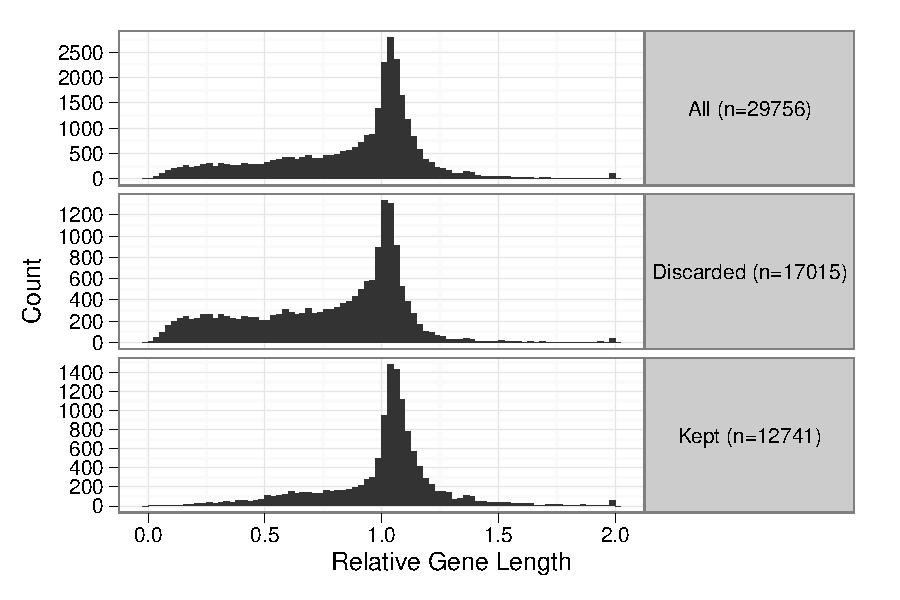
\includegraphics[scale=0.7]{Figs/filtered_paralogs_hist.pdf}
\caption{Gene lengths of all putative paralogs, normalized to the mean
  length all sequences in the enclosing tree of each
  paralog. Putatively paralogous genes (top panel) were either
  discarded (middle panel) or kept (bottom panel) according to rules
  based on their length and mean sequence divergence from other
  aligned sequences.}
\label{filtered_paralogs_hist}
\end{figure}

Figure \ref{filtered_paralogs_hist} shows the distribution of gene
lengths (relative to the mean across the alignment) for all putative
paralogs, kept paralogs, and removed paralogs. The overall
distribution of relative lengths shows that most putative paralogs had
lengths similar to the mean length across the gene tree (with a peak
at or slightly above 1), but the shape of the distribution was highly
asymmetric with a strong bias towards shorter lengths. The length
distribution of the retained paralogs showed that the bulk of
highly-shortened genes were successfully removed. If anything, the
distribution of retained genes was slightly biased towards lengths
greater than 1; this was likely due to step \#3 of the above process,
where the longest gene was kept if any two putative paralogs yielded
identical distance estimates.

\begin{figure}
\centering
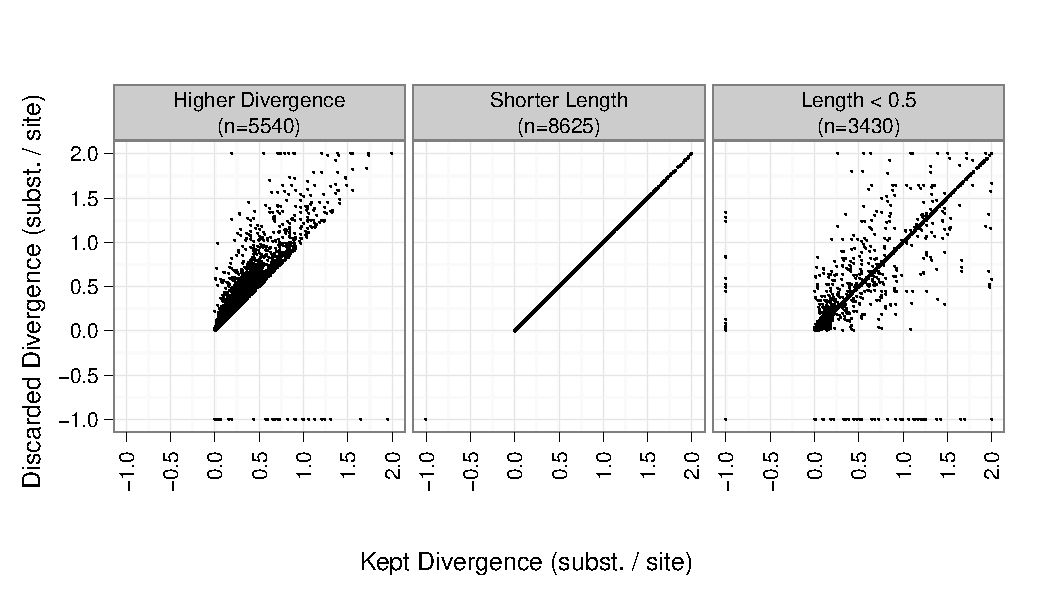
\includegraphics[scale=0.7]{Figs/filtered_paralogs_scatter.pdf}
\caption{Sequence divergence of kept and discarded putative
  paralogs. Each point represents a gene which was discarded from the
  tree for one of three reasons: it had more sequence divergence than
  the kept gene (\emph{Higher Divergence}; left panel), it had equal
  sequence divergence but shorter length than the kept gene
  (\emph{Shorter Length}; middle panel), or it had a gene length
  (relative to the mean across all sequences) of less than 0.5 while
  the kept copy had a relative length greater than 0.5 (\emph{Length
    $<$ 0.5}; right panel). Divergence was measured as the mean
  pairwise divergence between the gene and all other sequences in the
  tree, and a value of -1 was assigned to genes for which no reliable
  divergence estimate could be attained due to a lack of sufficient
  data)}
\label{filtered_paralogs_scatter}
\end{figure}

An alternate view of the results of the paralog filtering process is
shown in Figure \ref{filtered_paralogs_scatter}, with the mean
divergence of each discarded paralog compared that of the kept
paralog, separated into panels according to the reason for which the
discarded gene was removed. The spread of points above the diagonal in
the first panel shows the difference in mean sequence divergence
between the kept and discarded putative paralogs where divergence was
used to choose between copies, and the middle panel represents
paralogs whose mean divergences were identical, where length was used
as the deciding factor. These two panels together show that although
most recent paralogs within this set of gene trees contained
indistinguishable levels of sequence divergence, around 40\% showed a
moderate difference in divergences that could be used for selecting
the less-diverged copy. The rightmost panel shows the subset of
apparent paralogs which were discarded due to their short gene length;
a point worth noting here is that there was no bias towards higher or
lower divergence levels in this set of discarded genes (many of the
points lie directly on the diagonal, and the coefficient of the
best-fit linear model for all non-negative values was $0.983 \pm
0.005$), which was consistent with the prediction that many of the
discarded short genes were in fact derived from a single orthologous
gene.

\subsection{Realigning coding sequences}

After filtering out codons with low quality scores and removing
paralogs, sequences were aligned with \prank \citep{Loytynoja2008}
using its codon alignment model based on the empirical codon model
\citep{Kosiol2007}. The simulation experiments described in Chapters
\ref{ch_indels1} and \ref{ch_indels2} as well as numerous
previously-reported empirical and simulation-based studies have shown
\prank{}'s codon-based alignments to be superior for avoiding false
positives in the detection of sitewise positive selection, strongly
supporting the choice of \prank for this analysis.

\subsection{Filtering out clusters of \nsyn substitutions}

Manual analysis of a number of genes showed that even after 

A final filtering step was applied in order to ensure that stretches
of aligned but nonhomologous sequence, resulting either from
misalignment or from exon mis-annotation artifacts, were not causing
elevated rates of \nsyn substitutions within specific regions of
genes. This filtering step motivated by an observation that errors
resulting from either misalignment or exon mis-annotation would in
both cases lead to clustered regions of nonhomologous aligned
nucleotides and, correspondingly, clustered regions of elevated \nsyn
substitution rates. This clustering was expected because for both
misalignment and mis-annotation, the existence of one misaligned
column is not independent of nearby columns: for mis-annotation the
misalignment would span the entire length of the erroneously-annotated
exon, while the global nature of the progressive pairwise alignments
created by \prank{} (along with most other progressive alignment
programs) would cause any misalignment error to be tightly associated
with misalignment errors in nearby alignment columns.

These arguments suggested the possibility that clustered \nsyn
substitutions might be used as a signal to detect misaligned and
mis-annotated regions, but the utility of such a signal for filtering
alignments would also depend on the strength of error-caused \nsyn
clusters relative to the frequency of true \nsyn substitutions along a
given branch in the gene tree and to the tendency of those
substitutions to cluster together along the length of the protein
sequence. Clearly, sequences sequences separated by longer branch
lengths will show higher numbers of non-erroneous \nsyn substitutions,
possibly exceeding the number typically produced by alignment or
assembly errors, thus and reducing the ability to use substitution
clusters as a discriminating factor. Furthermore, \nsyn substitutions
have been shown to be significantly more clustered than expected by
chance in a number of genomic analyses of mammals and insects
\citep{Callahan2011,Bazykin2004,Wang2007}, causing some concern that a
filter based on detecting clusters of \nsyn substitutions might
attenuate the signal of true adaptive substitution that was one target
of the present study.



\draft{Write up the empirical investigation of \nsyn substitution clustering.}

\section{Genome-wide analysis of sitewise selective pressures in mammals}

\subsection{Mammalian species subsets for sitewise analysis}

The SLR method was applied sequentially to several species subsets of
each alignment of mammalian orthologs. For each subset, sequences
corresponding to species within the subset were extracted from the
alignment along with the corresponding \subtr and input to SLR. If
fewer than two sequences were available for a given subset, that
subset was skipped and its absence from the dataset was
recorded. Eight subsets in total were selected for analysis; the
species included in each subset and some phylogenetic measures of each
subset are listed in Table \ref{species_set_summary}.

Three subsets (Glires, Primates, and Laurasiatheria) were chosen
because they represent the three mammalian superorders with the
greatest taxonomic representation in Ensembl, providing an opportunity
to compare the molecular evolutionary dynamics of three monophyletic
mammalian groups containing varying levels of divergence, diverse
biological characteristics, and a number of high-quality reference
genomes. A fourth parallel mammalian subclade, named Atlantogenata and
consisting of sloth, armadillo, tenrec, elephant and hyrax, was also
included, but the monophyly of this group is still debated
\citep{Murphy2007,Churakov2009} and it contains only one high-coverage
genome. As such, it was not considered a primary target for the
mammalian superorder analysis.

Two larger species sets, Eutheria and Mammalia, were chosen for the
purpose of measuring average sitewise selective pressures with high
precision across a wider group of mammals. Using the Ensembl species
tree as a guide, the estimated total synonymous branch lengths spanned
by Ensembl species within Eutheria and Mammalia were 4.95 and 6.18,
respectively. Simulations performed by Anisimova and Yang
\citeyearpar{todo, Anisimova Yang 2002} and by myself in Chapter
\ref{ch_indels1} predicted that the greater amount of branch length in the
Eutherian and Mammalian trees---with two to three times the value of
1.71 for Laurasiatheria, the superorder with the largest total branch
length---would result in significantly higher levels of power and
accuracy for estimating sitewise \omg and detecting sitewise positive
selection. In this respect, Mammalia and Eutheria were more similar to
each other than to any of the superorders.

However, the Mammalia and Eutheria subsets differed markedly in a
different (and largely orthogonal) phylogenetic factor, the
evolutionary depths of their last common ancestors. Whereas the
ancestor of all Eutherian mammals lived ca. \draft{125} mya, the
Mammalian ancestor dates back to \draft{320} mya. This suggested that a
comparison between the sitewise results for the two groups might
provide useful insight into the general effect of adding longer,
deeper branches to a sitewise evolutionary analysis as well as some
indirect evidence on the molecular evolutionary dynamics of our most
distant mammalian relatives (the Eutheria and Mammalia groups only
differ by the inclusion of wallaby, opossum and platypus in the
Mammalia group).

Quantitatively, as measured by the \mpl from the Ensembl species tree,
the Eutheria subset (\mpl=0.24) is far more similar to either of the
three superorders (\mpl from 0.13 to 0.27) than to the Mammalia subset
(\mpl=0.54). This is due to the striking adaptive radiation of
Eutherian mammals \citep{Archibald1999,BinindaEmonds2007}, which
caused a quick succession of speciation events around the K-T boundary
and gives a largely star-like structure to the eutherian evolutionary
tree. Interestingly, according to the time-resolved mammalian tree
from Bininda-Edmonds et al. \citeyearpar{BinindaEmonds2007} the
Diprodontia order (containing wallaby and opossum, two outgroups to
the Eutheria clade) experienced a radiation similar to, but less
prounced than, the Eutherian radiation; a comparison of the evolution
of the deeply-rooted Diprodontia clade to its sister Eutherian clade
would be very enlightening, but the species representation of
Diprodontia (currently at one high-coverage and one low-coverage
genome) is too limited to allow for a powerful analysis. Nevertheless,
the inclusion of the three non-Eutherian species in the Mammalian
species group was expected to provide an additional data point for
aiding in an understanding of the complex relationship between branch
length, power and biological variability in the analysis of sitewise
selective pressures.

Finally, to further investigate the combined impact of evolutionary
depth, biological variability and branch length on the results of
large-scale sitewise analyses, two ``sparse'' subsets were created to
act as controls relative to two existing species subsets. The species
in the Sparse Glires group were chosen to approximate the total branch
length of the Primate clade with species from the Glires clade, while
the Sparse Mammals subset was constructed by selecting one species
(preferably with a high-coverage genome) from each major mammalian
branch, greatly reducing the total branch length covered but
maintaining a similar evolutionary depth and distribution of branches
within the species tree. The branch lengths in Table
\ref{species_set_summary} show that the Sparse Glires group was only
somewhat successful in its goal of approximating the Primates branch
length (with total branch lengths of 0.99 and 0.68, respectively)
while the Sparse Mammals group achieved a threefold lower total branch
length compared to the full Mammalia group while maintaining a nearly
identical \mpl.

% latex table generated in R 2.13.0 by xtable 1.5-6 package
% Thu Sep 15 11:19:59 2011
\begin{table}
\centering \footnotesize
\begin{tabular}{lb{6cm}rrrrr}
\toprule
 & &  & \multicolumn{2}{c}{Ensembl} & \multicolumn{2}{c}{Gene Median} \\
\cmidrule(r){4-5} \cmidrule(r){6-7}
Name & (Species Count) Species List & \Ne & MPL & Total & MPL & Total \\
  \midrule
\input{Tables/species_set_summary.txt}
\bottomrule
\end{tabular}
\caption{Species subsets used for sitewise analysis. Values under the
  ``Ensembl'' heading were calculated from subsets of the species tree
  used for evolutionary analyses by the Ensembl Compara pipeline,
  while values under the ``Gene Median'' heading were calculated as
  median values across the \ngenes gene trees analyzed (with branch
  lengths optimized by SLR). MPL -- mean path length, Total -- total
  branch length.}
\label{species_set_summary}
\end{table}

\subsection{Evaluation of the bulk distributions and the design of a filtering appraoch}

Sitewise data were collected from SLR and stored in a database for
storage and further analysis. The Mammalia subset, containing the most
branch length of all the datasets and representing the entire set of
aligned sequences, and the Primate subset, containing the lowest
overall branch length, were used to perform quality-control checks on
the sitewise data. The point of these checks were to evaluate whether
any additional filtering of the sitewise results was necessary before
characterizing the global distribution of constraint in this and the
other species subsets. Even if the sequence and alignment filters
described above were successful at reducing the number of false
positives due to incorrect input alignments, the behavior of SLR when
applied to large datasets of heterogeneous alignments has not been
well-studied, and a number of biases might have influenced the
results. A particular point of concern was that columns with different
patterns of gap and non-gap sequences, especially those with few
non-gap sequences, might yield different performance
characteristics. Although the SLR method was sensibly designed to
account for uncertainty in the estimation of \omg and detection of
positive selection, one might reasonably expect less-desirable
statistical properties from sites with 2 non-gap sequences compared to
sites with 20.

\begin{landscape}
\begin{figure}
\centering
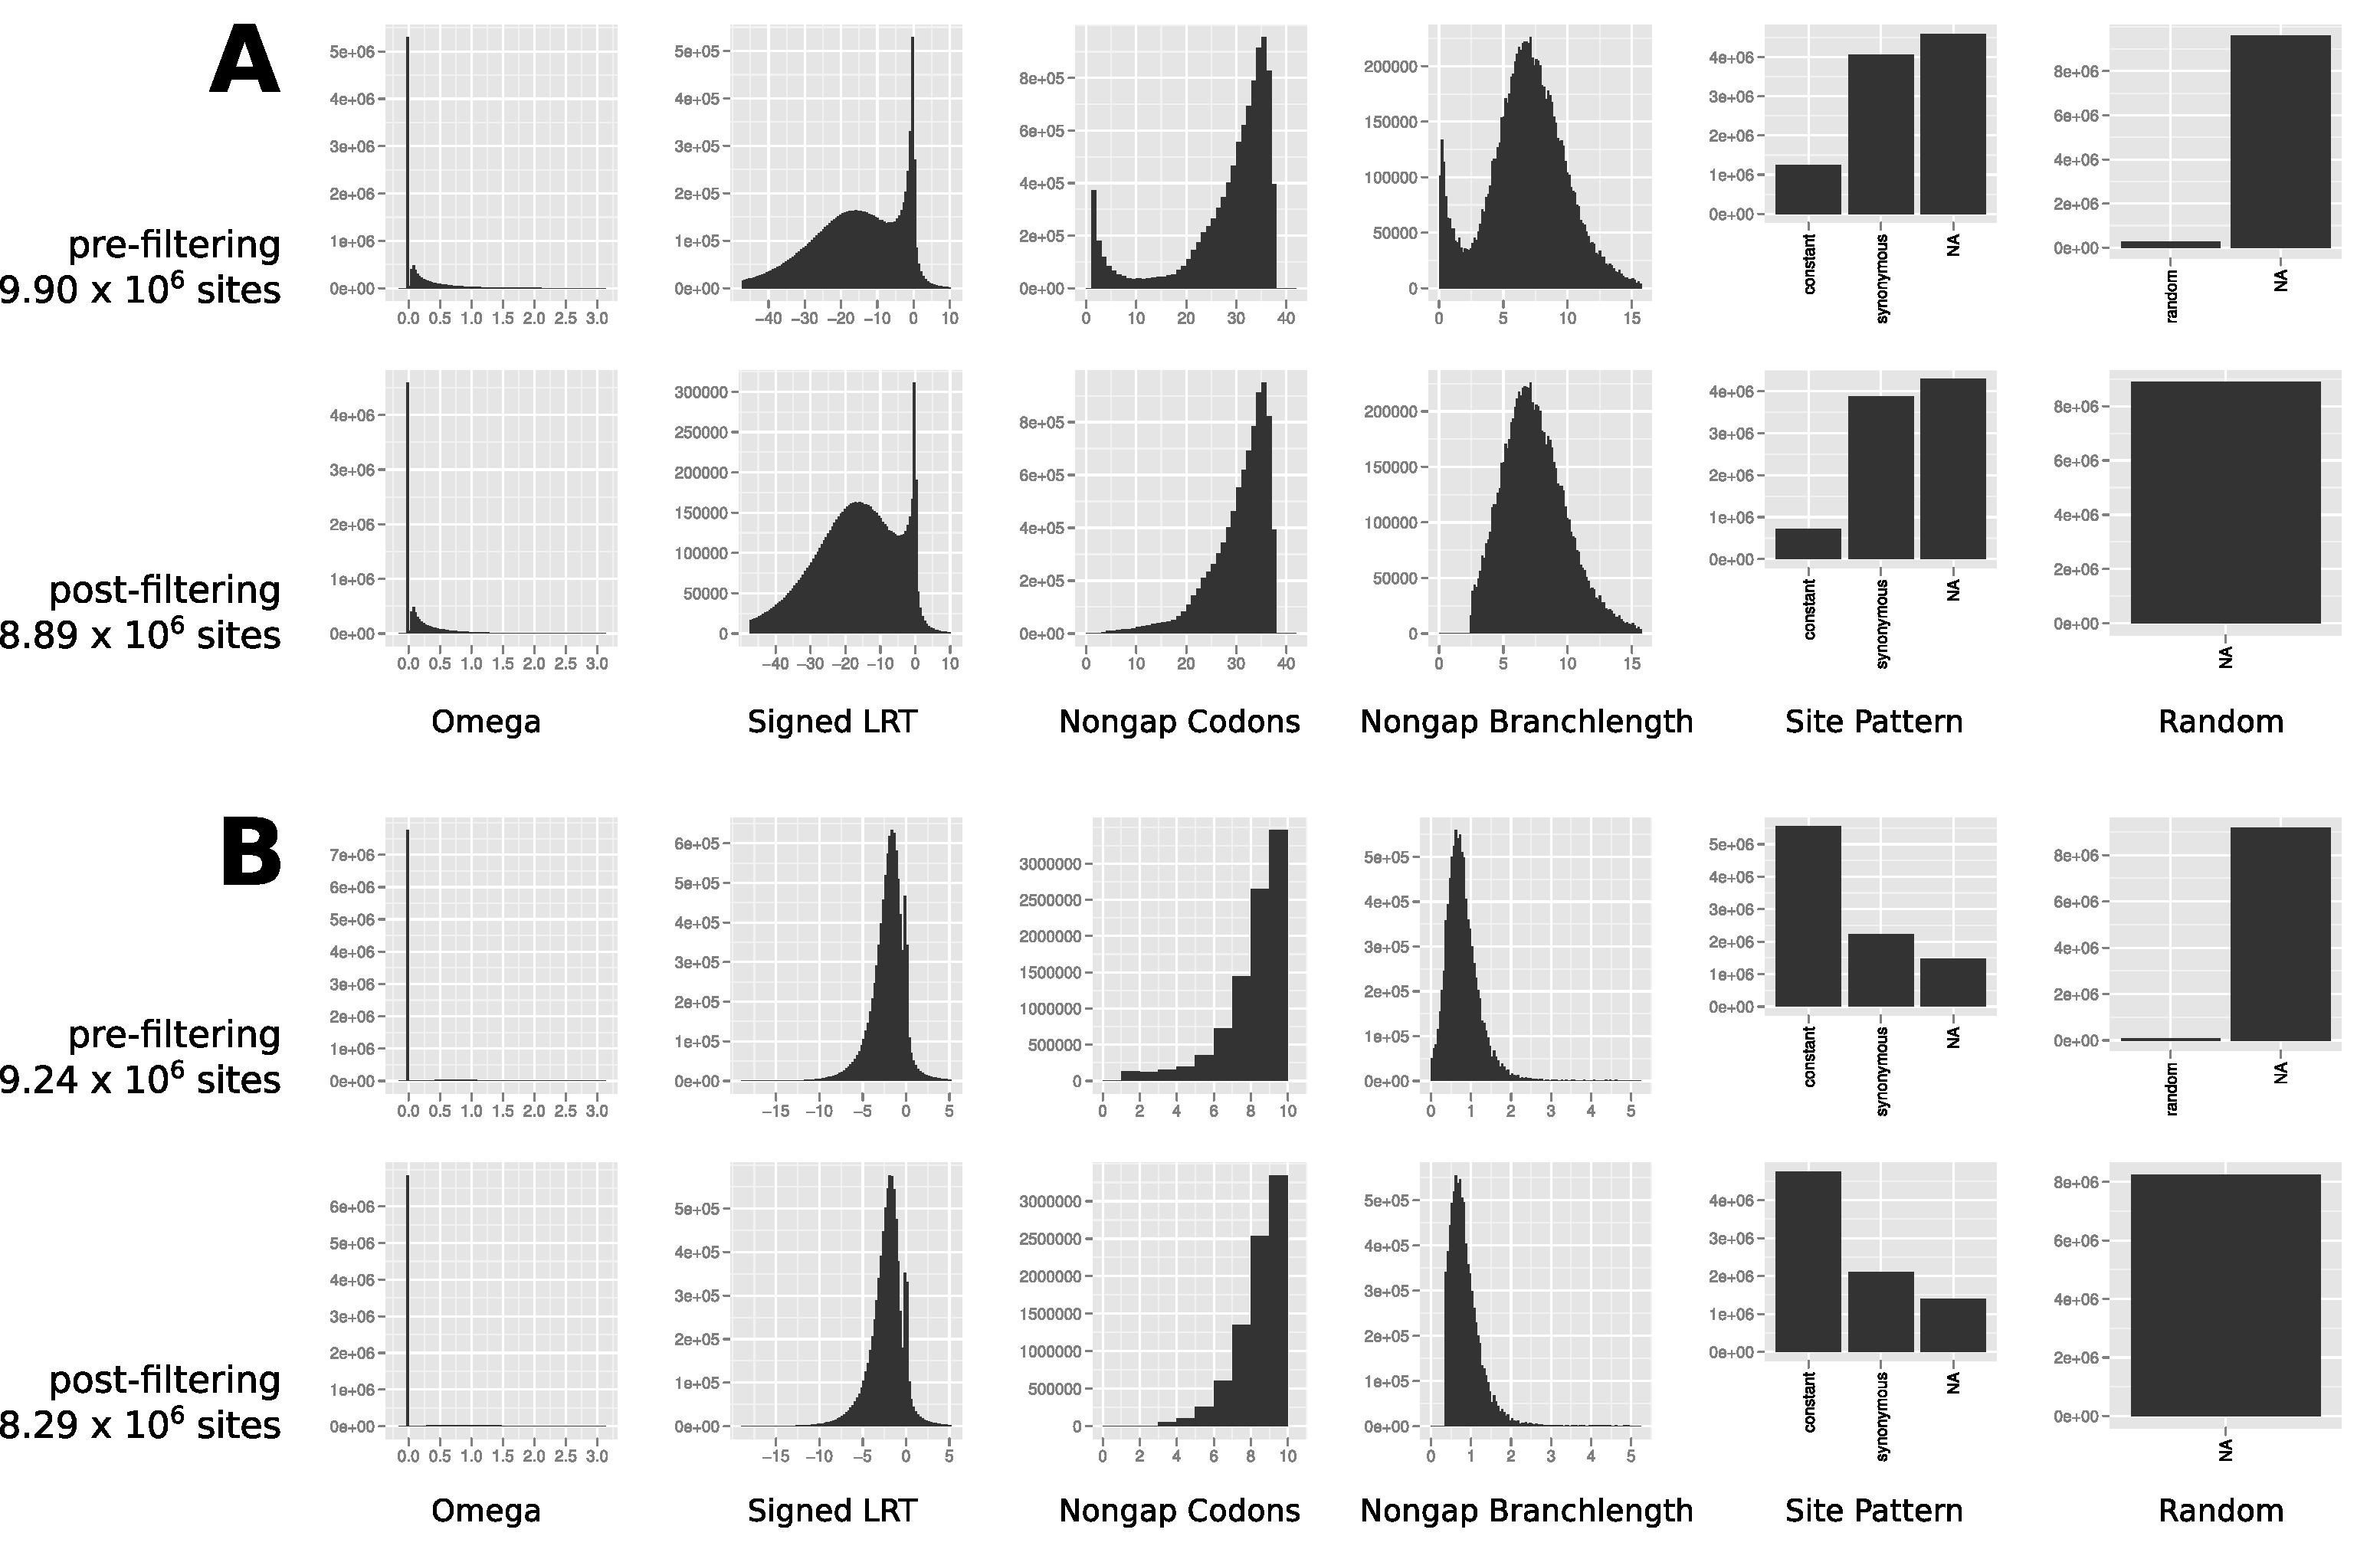
\includegraphics[scale=0.42]{Figs/qc_hist_mammals_primates.pdf}
\caption{Distributions of sitewise values for Mammalia (A) and (B)
  Primates, before (top row) and after (bottom row) removing sites
  based on the filtering scheme (see text). Note: the y-axis scale
  varies between rows, and the x-axis scale varies between (A) and (B)
  for the Signed LRT, Nongap Codons and Nongap Branch Length values.}
\label{qc_hist_mammals_primates}
\end{figure}
\end{landscape}
 
Figure \ref{qc_hist_mammals_primates} shows the distributions of six
sitewise values: two continuous values output by SLR (Omega and Signed
LRT), two categorical values from SLR (Site Pattern and Random), and
two values calculated from the codon alignment (Nongap Codons and
Nongap Branch Length). The Nongap Codons value measures the number of
non-gap codons in the given alignment columnn, while the Nongap
Branch Length represents the total branch length connecting all non-gap
sequences (using the gene tree with branch lengths optimized by SLR).

A prominent feature of the distribution of \omg values for the
unfiltered Mammalian data, shown in the top panel of Figure
\ref{qc_hist_mammals_primates}A, was the large number of sites with a
maximum-likelihood estimated \omg of zero. Further inspection of the
data revealed that all zero-\omg sites contained either \syn or
constant site patterns, and all sites with constant patterns (and
nearly all sites with \syn patterns) yielded a \ml \omg estimate of
zero. An estimate of zero for \syn sites is intuitively appropriate,
as the lack of any \nsyn substitutions throughout the tree would seem
to provide no evidence for a \nsyn substitution rate of greater than
zero. For constant sites the case is less clear, because no data
regarding the rate of either \syn or \nsyn substitutions
exists. However, given SLR's assumption of a constant \syn
substitution rate throughout each gene \citep{Massingham2005},
the \omg value which maximizes the likelihood of observing zero
substitutions is zero, since that value minimizes the \nsyn (and
total) substitution rate.

It is interesting to note that a small proportion (ca. 0.2\%) of \syn
sites resulted in \ml estimates greater than zero. Manual
investigation of a number of these sites \draft{Use the sites data and
  'seq' table to do a more quantitative analysis here?}  showed them
all to include synonymous codons with multiple nucleotide differences
(such as those coding for serine and arginine), for which SLR's
mechanistic codon model---which does not allow for multiple
simultaneous nucleotide changes--required the inference of multiple
\nsyn substitutions and, thus, a \nsyn substitution rate of greater
than zero. The existence of multiply-substituted codons in alignments
has been previously reported \citep{Averof2000,Whelan2004}, and
empirical results have supported the notion that codon models that
allow for multiple simultaneous nucleotide changes better describe
evolution than those that do not \citep{Kosiol2007}. However, the very
low proportion of synonymous sites requiring nonzero \nsyn
substitution rates suggested that the impact of these effects on the
current dataset was minimal; this is likely due to the relatively
short branch lengths separating the nodes of the mammalian tree,
making it less likely that codons with multiple substitutions (whether
the result of simultaneous multiple nucleotide changes or successive
single changes) would be observed \citep{Kosiol2007}.

The distributions of Nongap Codons and Nongap Branch Length values in
the top row of Figure \ref{qc_hist_mammals_primates}A showed that many
alignment columns contained only a few non-gap sequences. Both
distributions were bimodal with a larger peak at the upper end of the
range and a smaller peak at the lower end of the range. If the sites
with low non-gap codon counts represented accurate evolutionary
histories, the observed excess of mostly gapped sites might be taken
as an indication that insertion events in terminal lineages or recent
ancestral lineages were prominent enough in mammalian evolution to
leave a noticeable signature of sites with low non-gap codon
counts. This would be a very interesting observation, but
unfortunately it is not likely a correct one. Given the many possible
sources of error in the creation of Ensembl gene trees, however, a
more likely scenario was that sites with low codon counts and low
branch lengths came from stretches of sequence which only exist in a
few species as a result of annotation or alignment error, with a
higher probability of being nonhomologous and showing spurious signals
of positive selection. This would make such sites prime candidates for
filtering out prior to a large-scale analysis.

To test the hypothesis that sites with few non-gap sequences are less
reliable than other sites, the Mammals and Primates data were split
into deciles by nongap branch length and sites within each decile were
summarized by the proportion of sites showing evidence for purifying
and positive selection; the results of this analysis are presented in
Table \ref{bl_pos_sel_breakdown}. The lowest decile appeared to be a
clear outlier in the Mammalia dataset, with nearly 17\% of sites
having an estimated \omg of greater than 1 and 2\% of sites showing
significant evidence for positive selection at a nominal 5\% error
rate. Deciles with greater nongap branch lengths showed lower
proportions of sites with \omg $> 1$ and less evidence for positive
selection, with a gradual increase in both values at progressively
higher deciles. The gradual increase in evidence for positive
selection with increasing nongap branch length could be explained by
genes with higher overall \dnds ratios (and perhaps more positive
selection) producing, on average, higher estimated branch lengths due
to the increased \nsyn substitution rate. Overall, these patterns were
consistent with the expectation that sites with few non-gap sequences
were not consistent with the bulk of the dataset, and Table
\ref{bl_pos_sel_breakdown} showed that removing sites with the lowest
10\% of nongap branch length would remove most of the apparently
anomalous sites.

The breakdown of Primates data in Table \ref{bl_pos_sel_breakdown}
showed a trend similar the Mammalia dataset, although the distinction
between the lowest decile and the rest of the dataset was less
clear. The \fpos in the lowest decile was only slightly higher than in
the next-highest decile, and \fblw was lower than in all other
bins. The gradual increase of \fabv and \fpos in higher branch length
deciles was similar to that seen in the Mammalia dataset,
however. Despite weaker evidence in the Primates data for the
erroneous nature of sites with few non-gap sequences, it still
appeared that filtering sites in the bottom decile would improve the
overall quality and consistency of the data.

\begin{table}
\centering \footnotesize
\begin{tabular}{lrrrrrrrrrr}
\toprule
 & BL & \multicolumn{3}{c}{Nongap BL} & \multicolumn{3}{c}{Nongap Codons} & \multicolumn{2}{c}{\omgml, \%} &  \\
\cmidrule(r){3-5} \cmidrule(r){6-8} \cmidrule(r){9-10}
 & Quantile & 25\% & 50\% & 75\% & 25ff\% & 50\% & 75\% & $< 1$ & $> 1$ & \psfive, \% \\
  \midrule
\input{Tables/bl_pos_sel_breakdown.txt}
\bottomrule
\end{tabular}
\caption{Proportions of sites with evidence for purifying and positive
  selection in the Mammalia and Primates datasets broken down by
  nongap branch length. Sites were separated into 10 equally-sized
  bins of nongap branch length and summarized by the $25^{th}$,
  $50^{th}$ and $75^{th}$ percentiles of nongap branch length and
  nongap codons, the percentage of sites with \omg estimated below or
  above 1, and the percentage of sites with significant evidence of
  positive selection at a nominal 5\% FPR.}
\label{bl_pos_sel_breakdown}
\end{table}

Turning back to the bulk distributions in Figure
\ref{qc_hist_mammals_primates}, the rightmost panel depicts the small
set of sites designated as ``random'' by SLR. These sites were flagged
by SLR as having a site pattern not significantly different from
random \citep{Massingham2005}, and they were also targeted for
removal before analysis of the global distribution.

The final filtering protocol applied to each sitewise dataset included
three steps. First, all sites within the bottom 10\% of nongap branch
length values were removed; second, sites flagged by SLR as ``random''
were removed; third, all sites with fewer than four non-gap sequences
were removed.

The most prominent effect of the filter on the bulk distributions in
Figures \ref{qc_hist_mammals_primates}A and
\ref{qc_hist_mammals_primates}B was, as expected, the removal of the
excess of sites with low non-gap branch lengths and non-gap codon
counts. The distribution of \omg estimates and Signed LRT statistics
were largely unchanged, indicating that the overall characteristics of
each dataset were not significantly altered by the filter. The lack of
large-scale change was a somewhat reassuring result, given that the
filter only removed roughly 10\% of sites from each dataset.

A more detailed comparison of various summary statistics for the
filtered and unfiltered datasets showed that filtering had a
noticeable impact on three quantities of interest: it reduced the
proportion of constant sites, lowered the mean \omg, and slightly
decreased the percentage of positively-selected sites. Tables
\ref{sitewise_summary_table_1} and \ref{sitewise_summary_table_2}
contain summary statistics and calculations performed on the filtered
and unfiltered Mammalia and Primates data. Most of the data contained
in these tables will be more fully described in the next subsection,
but a comparison of the filtered and unfiltered rows for Primates and
Mammalia provided a means by which to quantitatively assess the effect
of filtering on particular aspects of the dataset. First, the
percentage of constant sites was reduced in the post-filtering data,
moving from 60.04\% to 57.62\% in Primates and from 12.62\% to 8.17\%
in Mammalia. This was expected, as the sites removed by filtering were
enriched in constant site patterns due to their lower non-gap branch
lengths. Second, the mean \omg value was slightly reduced in Primates
(from 0.32 to 0.27) and greatly reduced in Mammalia (from 0.49 to
0.20), likely due to the removal of sites containing a small number of
nonhomologous codons which might have produced abnormally high
sitewise \ml \omg estimates. Third, the proportion of
positively-selected sites (shown for a range of significance
thresholds in Table \ref{sitewise_summary_table_2}) was moderately
reduced in both Primates (from 0.56\% to 0.53\% at \chisqlt{0.05}) and
Mammalia (from 0.72\% to 0.56\%). These three effects of filtering,
each showing a shift indicating more useful data (e.g., a lower
percentage of constant sites) or less evidence for positive selection
(e.g., lower mean \omg and proportion of positively-selected sites) in
the post-filtering datasets, together provided evidence supporting the
inclusion of such a filtering step prior to the analysis and
comparison of sitewise estimates in different species sets. Although
most quantities of interest were not noticeably changed, those that
were affected by filtering shifted to more conservative values, which
was taken to be a positive sign given the persistent concern regarding
the presence of false positives in detecting positive selection.

\begin{landscape}
\begin{table}
\footnotesize{
\centering
\begin{tabular}{lllrrrrrrrrrrrrr}
\toprule
 &  & &  \multicolumn{3}{c}{Site Pattern, \%} & Med. & 
  \multicolumn{3}{c}{Nongap BL} & \multicolumn{2}{c}{\omgml} &
\multicolumn{4}{c}{\omgml Below / Above, \%} \\
\cmidrule(r){4-6} \cmidrule(r){8-10} \cmidrule(r){11-12} \cmidrule(r){13-16}
Name & Filter & Sites & Const. & Syn. & Nsyn. & Codons & Med. & Mean & SD & Mean & SD &
$< 0.5$ & $< 1$ & $> 1$ & $> 1.5$ \\
  \midrule
\input{Tables/filter_summaries_1.txt}
\bottomrule
\end{tabular}
\caption{Summary statistics and \ml \omg estimates for sitewise data
  in eight species groups. Rows labeled ``Primates (raw)'' and
  ``Mammalia (raw)'' were computed based on unfiltered data and are
  included for reference. Columns under the ``\omgml Above / Below,
  \%'' heading measure the cumulative percentage of sites with \omgml
  below or above the indicated value. Med.---median,
  Const.---constant, Syn.---\syn, Nsyn.---\nsyn, ML---\ml.
\label{filter_summaries_1}
}

\hspace{.2in}

\centering
\begin{tabular}{llrrrrrrrrrrrrrrrrrrrrr}
\toprule
 & & \multicolumn{8}{c}{Positively Selected Sites (\%)} &
\multicolumn{3}{c}{\chisqlt{0.1}, \%} &
\multicolumn{3}{c}{\chisqlt{0.05}, \%} \\
\cmidrule(r){3-10} \cmidrule(r){7-10} \cmidrule(r){11-13} \cmidrule(r){14-16}
Name & Filter & 
  \multicolumn{2}{c}{\chisqlt{0.1}} & \multicolumn{2}{c}{\chisqlt{0.05}} &
  \multicolumn{2}{c}{\chisqlt{0.01}}& \multicolumn{2}{c}{\bhfdr{0.05}} &
  Neg. & Neut. & Pos. & Neg. & Neut. & Pos. \\
%\cmidrule(r){2-3} \cmidrule(r){4-5} \cmidrule(r){6-7} \cmidrule(r){8-9}
\midrule
\input{Tables/filter_summaries_2.txt}
\bottomrule
\end{tabular}
\caption{Proportions of sites subject to positive, purifying and
  neutral selection at various \slrt thresholds. The
  Benjamini-Hochberg method \citep{Benjamini1995} was used to identify the
  \slrt threshold at which FDR$<$0.05. For columns under the headings
  ``\chisqlt{0.1}, \%'' and ``\chisqlt{0.05}, \%'', Pos. and Neg. are
  the percentage of sites with significant evidence for positive and
  negative selection, respectively, and Neut. is the percentage of
  ``neutral'' sites not showing significant evidence for non-neutral
  selection.}
\label{sitewise_summary_table_2}
}
\end{table}
\end{landscape}


\begin{landscape}
\begin{table}
\footnotesize{
\centering
\begin{tabular}{lllrrrrrrrrrrrrr}
\toprule
 &  & &  \multicolumn{3}{c}{Site Pattern, \%} & Med. & 
  \multicolumn{3}{c}{Nongap BL} & \multicolumn{2}{c}{\omgml} &
\multicolumn{4}{c}{\omgml Below / Above, \%} \\
\cmidrule(r){4-6} \cmidrule(r){8-10} \cmidrule(r){11-12} \cmidrule(r){13-16}
Name & Filter & Sites & Const. & Syn. & Nsyn. & Codons & Med. & Mean & SD & Mean & SD &
$< 0.5$ & $< 1$ & $> 1$ & $> 1.5$ \\
  \midrule
\input{Tables/pset_summaries_1.txt}
\bottomrule
\end{tabular}
\caption{Summary statistics and \ml \omg estimates for sitewise data
  in eight species groups. Rows labeled ``Primates (raw)'' and
  ``Mammalia (raw)'' were computed based on unfiltered data and are
  included for reference. Columns under the ``\omgml Above / Below,
  \%'' heading measure the cumulative percentage of sites with \omgml
  below or above the indicated value. Med.---median,
  Const.---constant, Syn.---\syn, Nsyn.---\nsyn, ML---\ml.
\label{filter_summaries_1}
}

\hspace{.2in}

\centering
\begin{tabular}{llrrrrrrrrrrrrrrrrrrrrr}
\toprule
 & & \multicolumn{8}{c}{Positively Selected Sites (\%)} &
\multicolumn{3}{c}{\chisqlt{0.1}, \%} &
\multicolumn{3}{c}{\chisqlt{0.05}, \%} \\
\cmidrule(r){3-10} \cmidrule(r){7-10} \cmidrule(r){11-13} \cmidrule(r){14-16}
Name & Filter & 
  \multicolumn{2}{c}{\chisqlt{0.1}} & \multicolumn{2}{c}{\chisqlt{0.05}} &
  \multicolumn{2}{c}{\chisqlt{0.01}}& \multicolumn{2}{c}{\bhfdr{0.05}} &
  Neg. & Neut. & Pos. & Neg. & Neut. & Pos. \\
%\cmidrule(r){2-3} \cmidrule(r){4-5} \cmidrule(r){6-7} \cmidrule(r){8-9}
\midrule
\input{Tables/pset_summaries_2.txt}
\bottomrule
\end{tabular}
\caption{Proportions of sites subject to positive, purifying and
  neutral selection at various \slrt thresholds. The
  Benjamini-Hochberg method \citep{Benjamini1995} was used to identify the
  \slrt threshold at which FDR$<$0.05. For columns under the headings
  ``\chisqlt{0.1}, \%'' and ``\chisqlt{0.05}, \%'', Pos. and Neg. are
  the percentage of sites with significant evidence for positive and
  negative selection, respectively, and Neut. is the percentage of
  ``neutral'' sites not showing significant evidence for non-neutral
  selection.}
\label{sitewise_summary_table_2}
}
\end{table}

\end{landscape}


\subsection{The global distribution of sitewise selective pressures in mammals}

\begin{figure}
\centering 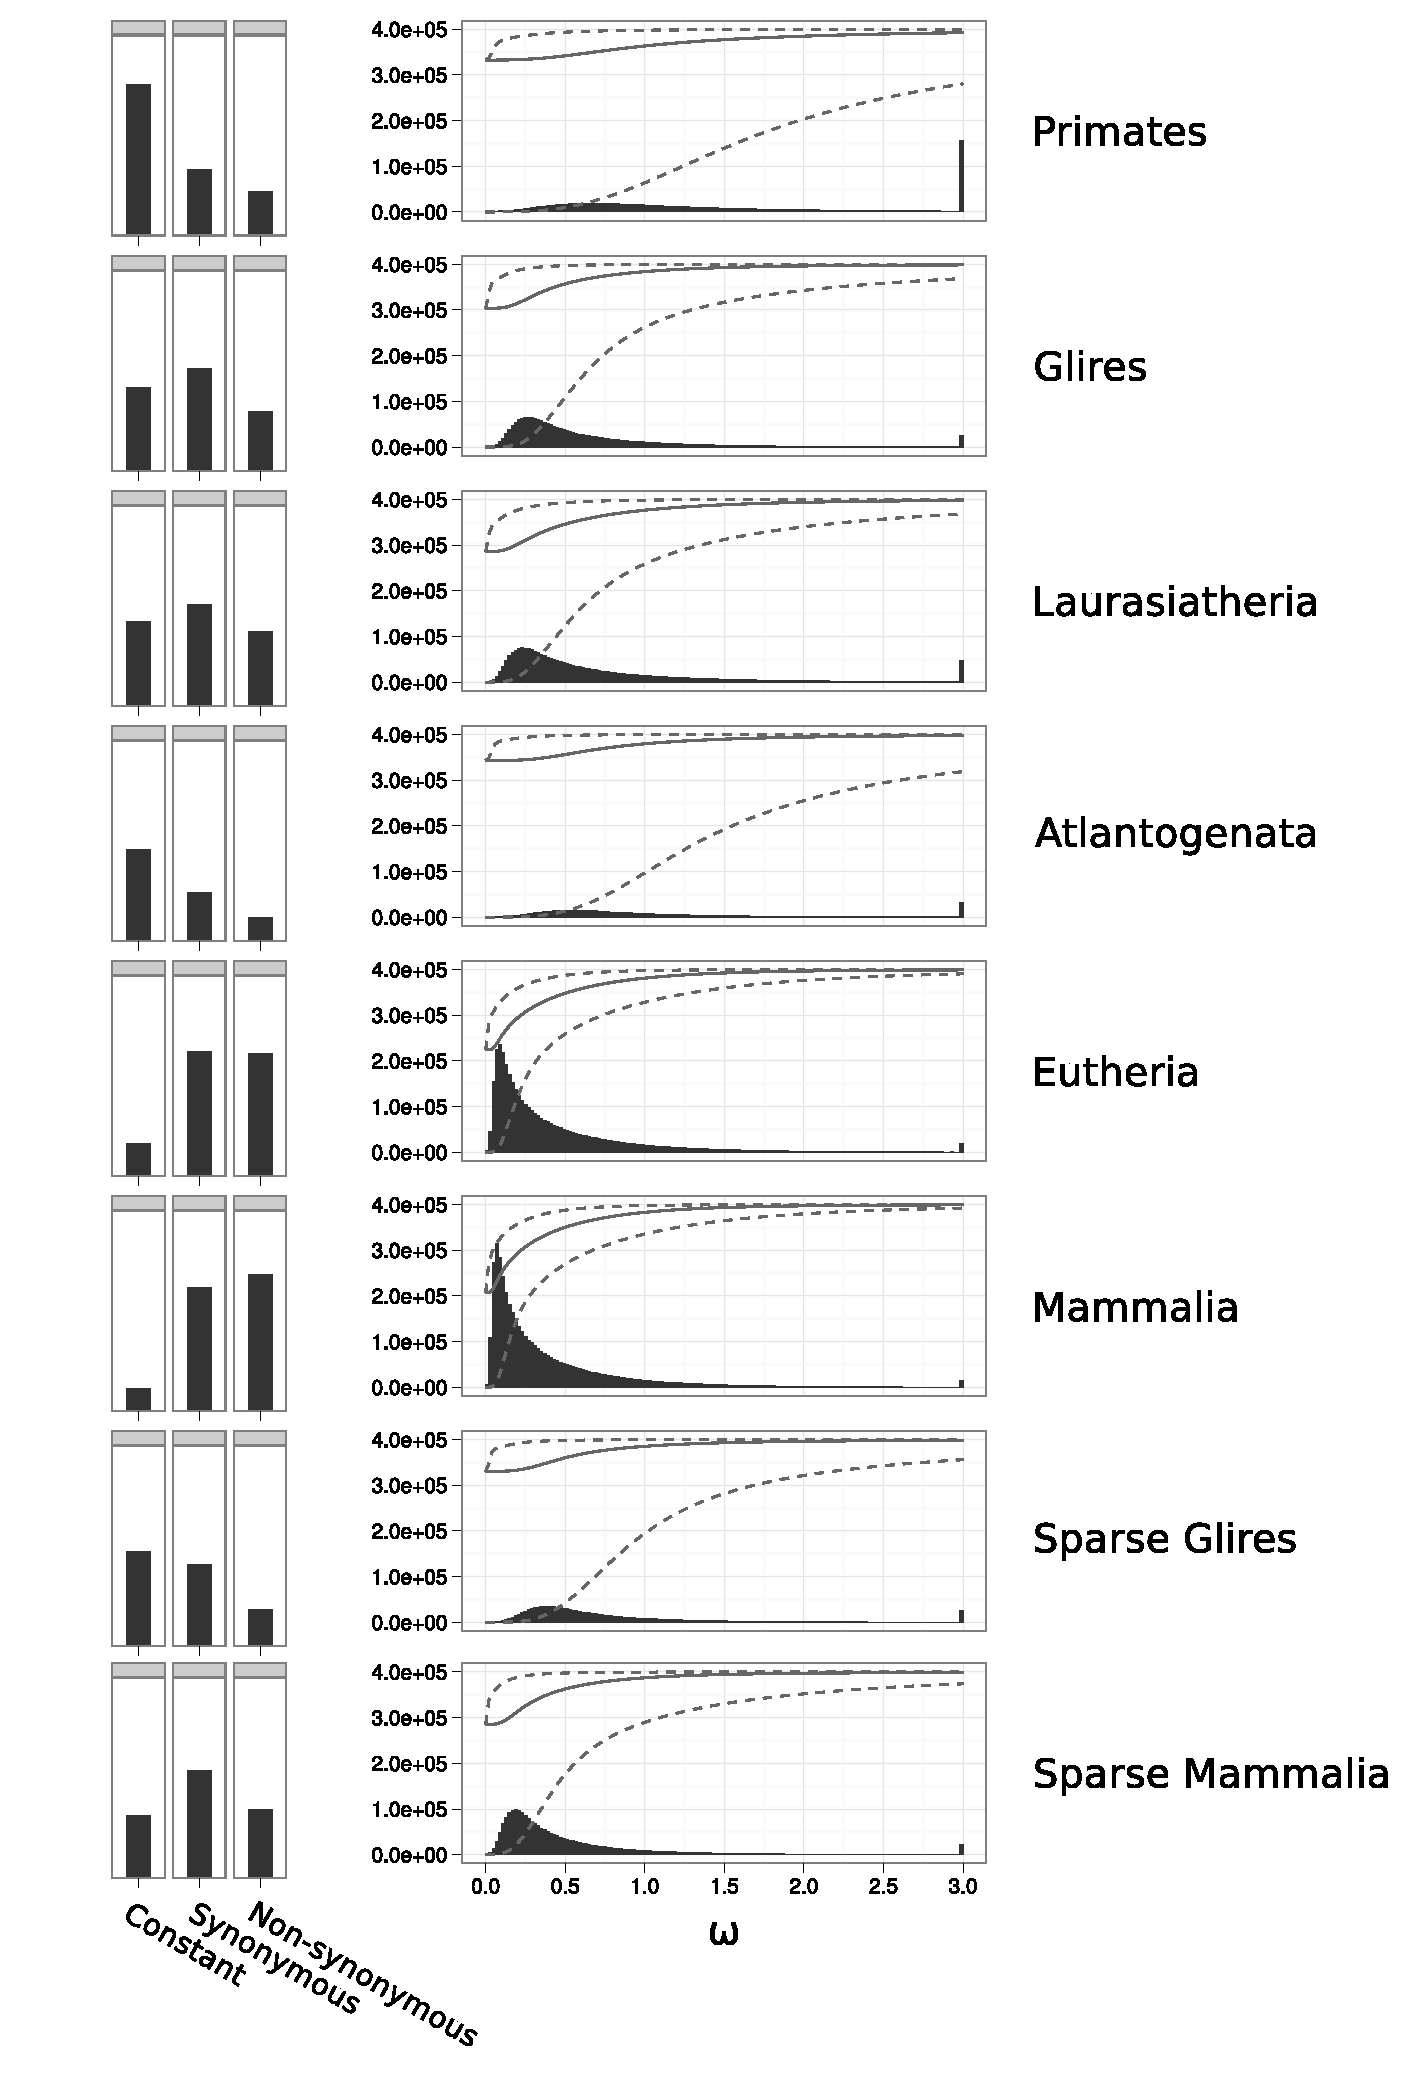
\includegraphics[scale=0.55]{Figs/global_distributions.pdf}
\caption{\scriptsize Global distributions of site patterns and \omg estimates for
  eight species groups. Left, bars represent the number of sites
  showing constant, synonymous, and non-synonymous patterns. Note, the
  y-axis is held constant between rows. Right, bars represent a
  histogram of \ml \omg estimates where $\omega>0$. Sites where
  $\omega>3$ are counted in the bin at $\omega=3$. A solid line is
  drawn showing the cumulative proportion of sites with \omg below the
  current value, and dashed lines are drawn above and below the solid
  line, showing the cumulative proportion of sites with the lower or
  upper range, respectively, of their 95\% confidence interval below
  the current value.}
\label{global_distributions}
\end{figure}

Each set of sitewise data was filtered as described above. The
resulting global distributions of site patterns, sitewise \omg
estimates, and 95\% confidence intervals are shown in Figure
\ref{global_distributions}; the left panel in each row plots the
number of sites with constant, \syn, and \nsyn patterns. All sites
with \omgml$=0$ had constant or \syn patterns, and all sites with
\omgml$>0$ had \nsyn patterns; the distributions of \omgml for these
\nsyn sites are shown as histograms on the right panel in each row.

\subsubsection{Site patterns and \omgml values reveal the prevalence of purifying selection in mammalian proteins}

The site pattern counts in Figure \ref{global_distributions} showed
that the branch length of each species group had a strong effect on
the overall composition of the sitewise data. Species groups covering
little branch length, such as Primates and Atlantogenata, contained a
majority of constant sites, while groups comprising lots of branch
length, such as Eutheria and Mammalia, contained few constant sites
and roughly equal proportions of \syn and \nsyn sites. Comparing the
Glires and Mammalia data with their corresponding ``sparse'' datasets
confirmed that this trend was largely due to branch length as opposed
to biological factors: the Sparse Glires data yielded a smaller
proportion of \nsyn sites and a greater proportion of constant sites
than the Glires data (17.41\% versus 24.08\% for \nsyn sites, 44.21\%
versus 33.98\% for constant sites; numbers from Table
\ref{sitewise_summary_table_1}), and the pattern for Sparse Mammalia
and Mammalia was qualitatively the same.

%I will cover the topic of branch length effects more thoroughly in the
%simulation study presented in Section \ref{poisson_sims}, but it
%should suffice to note here that the branch length covered by a given
%species group had a strong impact on the distribution of site patterns
%and the proportion of sites with \nsyn substitutions from which \nz
%\omg estimates could be made.

Turning to the distribution of these \omgml estimates, shown in Figure
\ref{global_distributions} as a series of histograms representing the
\omgml density (for \nz values only) and a series of solid lines
representing the cumulative density (for all values), it is clear
that the vast majority of protein-coding sites have evolved under
purifying selection in mammals. The Mammalia group, which contained a
very small proportion of potentially uninformative constant sites
(8.17\%), showed a maximum density of \nz \omgml estimates at
$\omega\approx0.1$, and the vast majority of sites showed some
evidence of purifying selection, with \omgml estimates below 1. The
height of the \omgml cumulative distribution at $\omega=1$ corresponds
to the proportion of such sites; the exact value, included in Table
\ref{sitewise_summary_table_1} under the ``$< 1$'' column, is
95.74\%. The \nz \omgml values were more evenly spread in the other
species groups, with Glires showing a maximum \nz \omgml density at
around $\omega\approx0.25$ and Primates at $\omega\approx0.7$. This
upwards shift in \nz \omgml estimates relative to Mammalia was likely
due to the greater proportion of constant and \syn sites in
lower-branch length datasets: sites which were truly evolving with
$\omega>0$, but where no \nsyn or \syn substitutions were observed,
would have their \omgml estimate ``pushed'' towards zero, causing an
increase in constant sites and a concomitant upwards shift in the
distribution of the remaining \nz \omgml values.

\subsubsection{Sitewise confidence intervals and LRT statistics identify sites with significant evidence for purifying and positive selection}

An important component of SLR's output is the set of statistics
providing information about the confidence with which purifying or
positive selection was detected. These values include the lower and
upper bounds of \ci, the 95\% confidence interval for each \omgml
estimate, and the LRT statistic, which corresponds to the strength of
evidence for purifying or positive selection. Following Massingham
\citeyearpar{Massingham2005}, I used a signed version of the
LRT statistic (hereafter \slrt), formed by negating the LRT statistic
for sites where \omgml$<1$, as a way to sort sites according to their
evidence, or lack thereof, for purifying and positive selection. Thus,
sites with \slrt$<0$ showed at least some evidence for purifying
selection and sites with \slrt$>0$ showed at least some evidence for
positive selection. It should be noted that the \slrt is a measure of
the strength of evidence for purifying or positive selection, but not
necessarily the actual strength of that selection. For example, an
alignment covering a very large branch length might yield a strongly
negative \slrt for a site with \omgml only moderately below 1, because
the difference between dN and dS was highly statistically significant;
on the other hand, a strongly-purifying site in an alignment covering
less branch length might produce a much less-negative \slrt, even with
\omgml near zero.

Figure \ref{sites_scatters}A shows the empirical relationship between
\slrt, \omgml and the \ci width for sites from the Mammali
dataset. The left panel, comparing the \slrt to \nz \omgml estimates,
shows that the two values are highly correlated, with the greatest
number of low \omgml estimates occurring at sites with strongly
negative \slrt{}s. Correspondingly, the middle panel shows an even
stronger relationship between the \slrt magnitude and the \ci width,
with the tighest windows at sites with very strong evidence for
purifying selection. The rightmost panel compares the \omgml of each
site with the width of its \ci, revealing a more linear and diffuse
positive relationship between \omgml and the size of the \ci. The
equivalent plots for Primates, shown in Figure \ref{sites_scatters}B,
reveal similar patterns, but with more weight towards less-negative
\slrt values, higher \omgml, and larger \ci. These differences
highlight the impact of branch length on the amount of confidence with
which \omg can be estimated, showing that the low branch length of the
Primates clade rarely yields \omgml estimates with \ci intervals
smaller than 1, while the bulk of sites from the Mammalia dataset have
a relatively small \ci. Thus, the \omgml distribution from datasets
with low branch lengths (e.g., Figure \ref{global_distributions})
should be interpreted with caution, and any comparison between
different sites or datasets must be sensitive to the amount of
statistical confidence placed on each estimate.

\begin{figure}
\centering
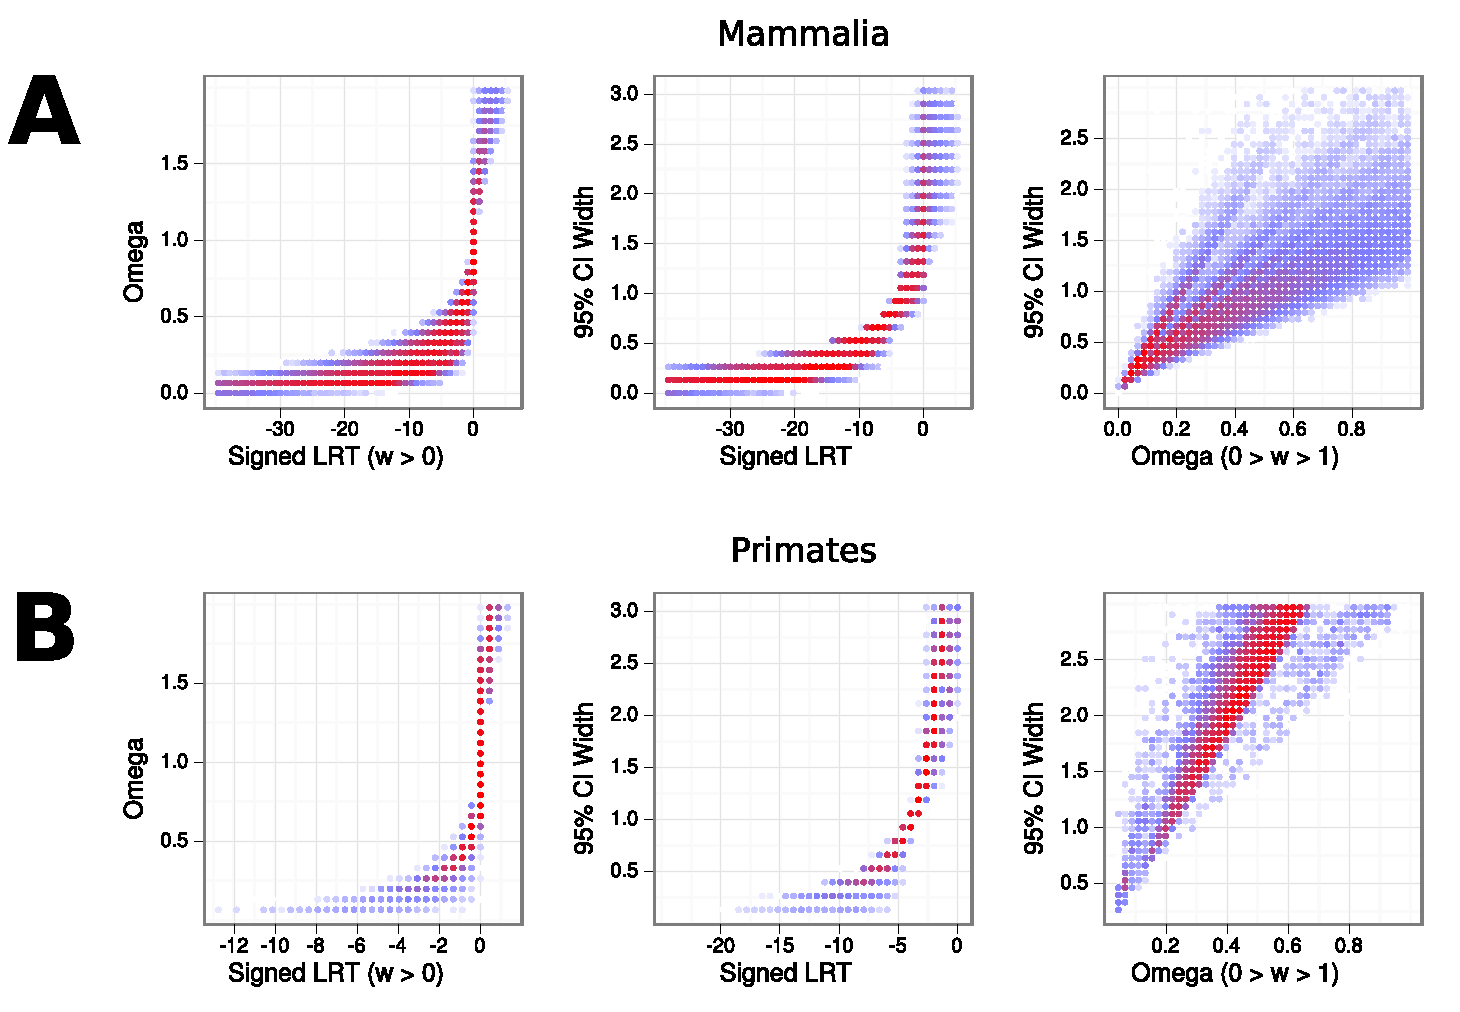
\includegraphics[scale=0.6]{Figs/sites_scatters.pdf}
\caption{The relationship between \slrt, \omgml, and \ci width in (a)
  Mammalia and (b) Primates datasets. Each point represents the binned
  density of sites; no points are drawn where no density exists, while
  blue and red points are drawn at areas of low and high density,
  respectively. The left panel shows sites where \omgml$<0$, the
  middle panel shows all sites, and the right panel shows sites where
  $0<$\xspace\omgml$<1$. Note the change in x-axis scale between plots
  in (a) and (b), reflecting the paucity of sites in Primates with
  strong evidence (\slrt$<$-12) for purifying selection.}
\label{sites_scatters}
\end{figure}

The statistical information at each site could be used to identify
sites evolving under purifying or positive selection with statistical
confidence. Sites with a \ciup, the upper bound of the \ci interval,
below \omg$=1$ showed evidence of purifying selection with an expected
5\% \fpr, and sites with a \cidown above \omg$=1$ showed evidence of
positive selection with an expected 5\% \fpr. In both cases, the 5\%
\fpr was expected under SLR's null model of neutral evolution. There
was a strong relationship between \ciup and the \chisq approximation
to the \slrt distribution, whereby the set of sites with \ciup$<1$ was
exactly equivalent to the set of sites with \slrt below the negative
\chisq 95\% critical value. Similarly, the sites with \cidown$>1$ were
those with \slrt above the \chisq 95\% critical value. Because of this
equality, I will refer to \slrt values instead of \ci intervals when
discussing sites with significant evidence for purifying or positive
selection. In some cases, however, use of the full \ci will be
preferable, as the \slrt critical values only correspond to one end of
the \ci, depending on whether the site shows greater evidence for
purifying or positive selection.

Table \ref{sitewise_summary_table_2} summarizes the results from using
the \chisq approximation to the \slrt distribution to identify sites
subject to purifying selection and positive selection at various \fpr
thresholds. The left group of columns show the number and proportion
of sites with evidence for positive selection at nominal 10\%, 5\%,
and 1\% \fpr thresholds, respectively, as well as an expected 5\% FDR
calculated using the Benjamini Hochberg method for FDR control
\citep{Benjamini1995}. The two groups of columns on the right show
the result of breaking sites into three groups (positive, negative,
and neutral) based on the result of a \chisq test at a given \fpr
threshold.

The positive selection results demonstrated that between 0.2\% to 1\%
of sites could be identified as under positive selection in mammals at
nominal FPR thresholds, but different species groups yielded
strikingly different estimates of the proportion of
positively-selected sites. At a 5\% FPR threshold, Primates,
Laurasiatheria, Eutheria, and Mammalia produced roughly comparable
proportions of positively-selected sites, ranging from 0.43\% to
0.72\%. The proportions of positively-selected sites in these groups
were higher using a 10\% FPR threshold (ranging from 0.70\% to 0.97\%
of sites) and lower using a 1\% FPR threshold (ranging from 0.14\% to
0.28\%). When the FDR was controlled using the Benjamini-Hochberg
method, however, only the Eutheria and Mammalia groups yielded a
substantial number of positively-selected sites; the Primates and
Laurasiatheria data were likely limited in their power to yield
positively-selected sites after FDR control due to their lower total
branch lengths. Interestingly, the Glires, Atlantogenata, Sparse
Glires and Sparse Mammalia datasets produced much lower proportions of
positively-selected sites across all \fpr thresholds. At FDR$<$0.05,
all four groups yielded zero significant \psc{}s.

In Mammalia, the breakdown of sites into positive, negative and
neutral categories at both \fpr thresholds produced a pattern similar
to the \omgml distribution, with overwhelming purifying constraint
(83.87\% of sites at 5\% FPR), a small proportion of
neutrally-evolving sites (15.57\%), and a small fraction of
positively-selected sites (0.55\%). As expected given the use of a
fixed \slrt threshold to identify purifying sites, the fraction of
sites confidently identified as under purifying selection showed a
strong dependency on the branch length of the species set, with a much
higher power in Mammalia than in Primates (83.87\% vs. 15.97\%).

Even for the Mammalia dataset, which encapsulated roughly 7.5
synonymous substitutions per site on average, one might reasonably
expect that the power to confidently identify sites under purifying
selection, though higher than in Primates, was still less than
100\%. If this is the case, then the proportion of confidently
identified purifying sites must be an underestimate of the true
proportion of negatively-selected sites (and by symmetry, absent any
methodological bias, the same should be true for positively-selected
sites). As a result, the fractions of positively- and
negatively-selected sites in Table \ref{sitewise_summary_table_2}
should not be taken as best estimates of the actual proportions of
such sites, but more appropriately as lower bounds on those
proportions. In fact, In the next two sub-sections, I will separately consider
the issue of using the sets of sitewise estimates in different species
groups to estimate the proportion of sites subject to purifying and
positive selection in mammals.

\subsubsection{Estimating the proportion of negatively-selected sites}

For sites under purifying selection, 

In , the value of $\approx$95\% based on \omgml$<1$ (Table
\ref{sitewise_summary_table_1}) is likely closer to the true number;
despite the caveats involved in ignoring the uncertainty involved in
\omgml estimates, the 95\% number was surprisingly consistent across
different species groups and branch lengths, ranging from
$\approx$91\% in Primates to $\approx$97\% in Sparse Mammalia.

\subsubsection{Estimating the proportion of positively-selected sites}

The pattern of the prevalence of positive selection across species
groups was surprising. First, 

, showing no sign of the expected correlation with
branch length. Theory predicts, and many studies have confirmed
\citep{Anisimova2001,Anisimova2002,Massingham2005}, that the power of LRT-based tests
for non-neutral selection should increase with branch length, as the
discrimination between \nsyn and \syn substitution rates becomes more
confident with more fixed substitutions. This was certainly the case
for identifying purifying selection, but there was no obvious
correlation between higher branch lengths and higher numbers of
confidently identified \psc{}s.

\subsubsection{Correlations between branch length, effective population size and sitewise summary statistics}

% Gotta look at these guys for Ne approximations: 
% http://www.pnas.org/content/104/51/20443.full

To quantify this observation, Spearman's rank correlation coefficients
between the median branch length of each species set and each of
several summary statistics were calculated (Table
\ref{summary_correlations}). Although the number of samples was small
with only eight species groups, these correlations should be able to
provide some indication as to which aspects of the sitewise data might
be easily attributed to the effects of branch length and which aspects
suggested an alternative (e.g., biological or artefactual) cause for
the differences between species groups. The results were quite
striking: the site classifications (constant, \syn and \nsyn) and the
proportion of negatively-selected sites at \chisqlt{0.05} were
strongly correlated with branch length, while the other factors,
including mean \omgml, the proportion of sites with \omgml$<1$ and
\omgml$<0.5$, and the proportion of positively-selected sites, were
weakly correlated or largely uncorrelated with branch length.

The results in Table \ref{summary_correlations} can be interpreted
in a number of ways. First, they emphasized the unambiguous
correlation between the branch length in a tree and the power to
detect sitewise purifying selection. However, they also showed that
various measures based on sitewise estimates contained variation
between species groups that was not well-explained by branch length. 

\begin{table}
\centering \footnotesize
\begin{tabular}{lrrrr}
\toprule
 & \multicolumn{2}{c}{Branch Length} & \multicolumn{2}{c}{\Ne} \\
\cmidrule(r){2-3} \cmidrule(r){4-5}
Value & Rho & P-value & Rho & P-value \\
\midrule
\input{Tables/summary_correlations_touchedup.txt}
\bottomrule
\end{tabular}
\caption{Correlations between median non-gap branch length, \Ne, and
  various summary statistics of the sitewise data across eight species
  sets. The magnitude (Rho) and significance (P-value) of Spearman's
  rank correlations between variables were calculated using \Ne values
  from Table \ref{species_set_summary} and branch lengths and summary
  statistics from Tables \ref{sitewise_summary_table_1} and
  \ref{sitewise_summary_table_2}. All summary statistics except for
  mean \omgml were measured as a fraction of total sites. More highly
  significant correlations are shaded in darker blue. \Ne{} -- estimated
  effective population size, BL -- non-gap branch length, \psfive
  -- positively-selected codons at \chisqlt{0.95}.}
\label{summary_correlations}
\end{table}



\subsection{Modeling the global distribution of sitewise selective pressures}
\label{modeling_distr}


\begin{landscape}
\begin{table}
\centering \footnotesize
\begin{tabular}{llrrrrrrrrrrrrrrr}
\toprule
 &  
 & \multicolumn{2}{c}{Log-normal} 
 & \multicolumn{2}{c}{Gamma} 
 & \multicolumn{2}{c}{Exponential} 
 & \multicolumn{2}{c}{Beta} 
 & \multicolumn{2}{c}{Weibull} \\
\cmidrule(r){3-4}
\cmidrule(r){5-6}
\cmidrule(r){7-8}
\cmidrule(r){9-10}
\cmidrule(r){11-12}

Species Set & Data Type
 & \omgmean & \% $>1$
 & \omgmean & \% $>1$
 & \omgmean & \% $>1$
 & \omgmean & \% $>1$
 & \omgmean & \% $>1$
\\
  \midrule
\input{Tables/distribution_fits.txt}
\bottomrule
\end{tabular}
\caption{Mean \omg and the percentage of sites with \omg$>1$ based on
  maximum-likelihood fits of parametric distributions to sitewise
  estimates. For each species set and each one of five distribution
  types (log-normal, gamma, exponential, beta, and weibull) 100
  replicate datsets of 1 million sites were sampled with replacement
  from the genome-wide dataset and the maximum likelihood distribution
  parameters were numerically optimized (see text for
  details). Columns show, for each distribution, the median value
  across 100 replicates of mean \omg (\omgmean) and the probability
  mass with \omg$>1$, expressed as a percentage (\%$>1$). The top
  eight rows show the results based on fitting parameters to sitewise
  \omgml estimates, and the bottom eight rows show the results based
  on fitting parameters to sitewise \ci estimates. Note the greater
  consistency of \omgmean and \%$>1$ across distribution types for the
  \ci{}-based fits.}
\label{distribution_fits}
\end{table}
\end{landscape}


\begin{table}
\centering \footnotesize
\begin{tabular}{llrrrr}
\toprule
Species Set & Distribution & AIC & $d$AIC & Parameter A & Parameter B
\\
  \midrule
\input{Tables/distribution_params.txt}
\bottomrule
\end{tabular}
\caption{ \scriptsize AIC values and parameters for maximum-likelihood fits of
  parametric distributions to sitewise \ci estimates. Distributions
  were fit to 100 replicate datasets for each species set as in Table
  \ref{distribution_fits}. For each species set and distribution type,
  the median Akaike information criterion (AIC) and parameter
  estimates are shown. Distributions are sorted according to their
  median AIC value (where a lower AIC corresponds to a better fit to
  the data), and the difference in AIC to the next-best fitting
  distribution is displayed ($d$AIC). The lognormal and beta
  distributions are ranked first or second in the mammalian superorder
  subgroups, while lognormal, weibull and gamma distributions fit the
  Eutheria and Mammalia datasets best. The named parameters
  corresponding to parameters A and B for each distribution are as
  follows: lognormal (A=meanlog, B=sdlog), weibull (A=shape, B=scale),
  gamma (A=shape, B=rate [where rate=$1/$scale]), beta (A=shape1
  [$\alpha$], B=shape2 [$\beta$]), exponential (A=rate [$\lambda$]).}
\label{distribution_params}
\end{table}

\begin{figure}
\centering
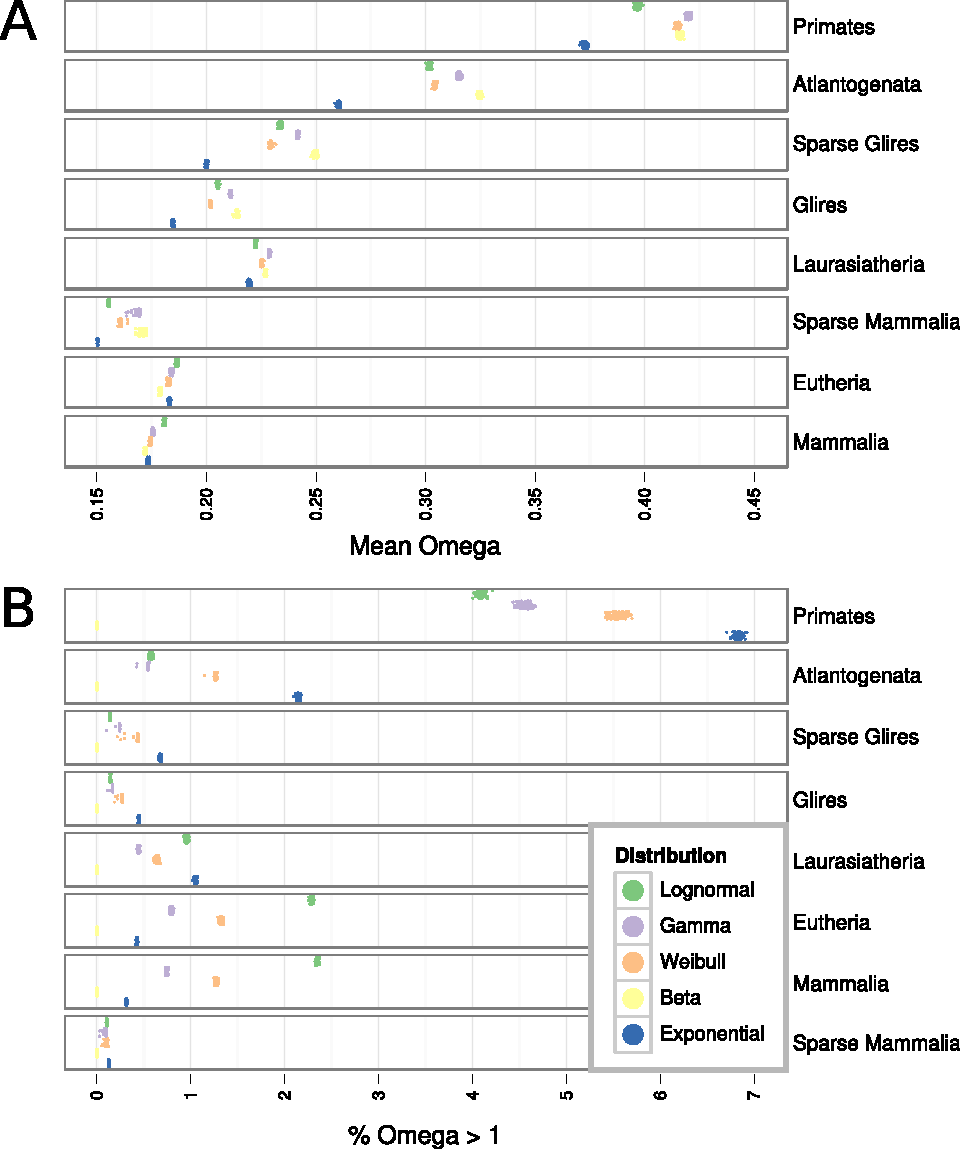
\includegraphics[scale=0.85]{Figs/distribution_fit_plots.pdf}
\caption{The mean value (A, Mean Omega) and the percentage of probability
  density with \omg$>1$ (B, Omega$>1$) from \ml fits of parametric distributions to
  sitewise \ci estimates. Each point represents the \ml fit of one
  distribution to 1 million points sampled from the genome-wide
  dataset with replacement; 100 such fits were generated for each
  distribution and species set. Note that the beta distribution is
  only defined on the interval (0,1), so the percentage of sites with
  \omg$>1$ was always zero.}
\label{distribution_fit_plots}
\end{figure}


% From 2xmammals supp. materials.
% https://docs.google.com/leaf?id=0B5HhSYGuKPKpYTY1YzVjNTgtODc2Yy00NzQ0LTgwZTQtMTQ3ZTA5ZWJjZGJm&hl=en_US
We used the ‘fitdistr’ function of the MASS package for R to fit five
distributions (gamma, lognormal, beta, Weibull, and exponential) to
the vertebrate dN/dS values and subsequently calculated Akaike’s
Information Criterion(AIC) for each fit. For all optimizations, a
constant value of 0.001 was added to sites where dN/dS = 0 in order to
satisfy the optimizer’s requirement that the probability functions
have a defined value for all input data. Similarly, sites with dN/dS ≥
1 were excluded from the analysis for the beta optimization. All
distributions were also separately fit to the subset of sites with
dN/dS ≥ 1; the AIC values from these optimizations were used to
compare the fit of the beta distribution to the others.

The fitdistr produced the following optimized parameters for each
function: gamma (shape=0.271, rate=1.203), lognormal (meanlog=-4.079,
sdlog=2.863), beta (shape1=0.257, shape2=1.431), Weibull
(shape=0.3882, scale=0.07151) exponential (rate=4.441). The beta
distribution yielded the lowest AIC when compared to the fit of other
distributions to the subset of sites where dN/dS ≤ 1 (-2.33e7 versus
the next best equivalent AIC of -2.11e7 for the lognormal). Of the
distributions which were fit to the whole dataset, the lognormal
distribution yielded the lowest AIC (-2.11e7), followed by gamma
(-2.03e7) and exponential (-6.45e6).

%\subsection{Analysis of sitewise estimates from the mammalian superorders}

\subsection{Simulations to evaluate the fit of empirical data to a simulated poisson process at varying branch lengths and \omg ratios}
\label{poisson_sims}

The large difference in branch lengths covered by the species sets
under investigation letd to some uncertainty in whether differences in
the observed summary statistics, such as the mean \omgml or the
proportion of sites with \omgml$<1$, were due to biological
differences between species groups (i.e., differences in the efficacy
of purifying selection resulting from population size differences) or
to branch length effects. For example, two 

I performed a small simulation
study to further investigate the interactions between branch length,
effective population size, and the summary statistics presented in
Table \ref{sitewise_summary_table_1},


\subsection{Simulations to evaluate the power to detect positive selection and estimate selective pressures}

% Table: https://docs.google.com/viewer?a=v&pid=explorer&chrome=true&srcid=0B5HhSYGuKPKpN2M0YzA5ZDQtN2FiNC00N2FhLWI0MzMtYjkwZTJmMjg2YmE5&hl=en

% Text from: https://docs.google.com/document/d/1H0hBD75a2fGmJL8l0BPQQPkcmpc6jmyT3Qr8g2zUV4A/edit?authkey=CKPKivsO&hl=en_US&authkey=CKPKivsO

Previous simulations on the power and accuracy of maximum-likelihood
methods for detecting sitewise positive selection have provided strong
evidence for increased power with increased branch length and number
of taxa [Anisimova and Yang 2002 PMID:12032251, Massingham and Goldman
  2005 PMID:15654091]. Other major effects observed have been a
reduction in power when branch lengths are very short, due to the
scarcity of data in the form of observed substitutions, and a
reduction in accuracy when branches are very long and the ancestral
reconstruction procedure becomes inaccurate due to saturation of
substitutions at synonymous sites [Anisimova and Yang 2002
  PMID:12032251]. These results have provided general guidance to
empirical analyses, but the potential effects of tree shape,
divergence level, distribution of dN/dS levels, and misalignment error
make it difficult to extrapolate expected power levels or error rates
from generic simulations to specific empirical analyses and real-world
datasets. In order to estimate the power of the SLR method when
applied to the present set of species and to quantify the power gained
from the additional 20 mammalian genomes, we ran a series of
simulation experiments with parameters tuned specifically to the
analysis of mammalian gene families. Based on the prevoius studies
described above we hypothesized that the addition of 20 mammalian
genomes to the available dataset would significantly improve SLR’s
sensitivity for detecting positive selection at a reasonable error
rate, with some portion of that improvement coming from a reduction in
alignment error due to the shorter average length of branches in the
phylogenetic tree being aligned.

We used the Indelible program [Fletcher and Yang 2010 PMID:19423664]
to simulate 100 replicate codon alignments with a root sequence length
of 500 codons for each of three trees: all 29 Eutherian mammals, the 9
mammals with high-coverage genomes, and the four-species
Human-Mouse-Rat-Dog quartet used in a number of previous comparative
analyses. The dN/dS value at each simulated site was drawn from a
discretized lognormal distribution with log(mean)=-1.864 and
log(sd)=1.201 with the maximum dN/dS capped at 3. This distribution
yielded a mean dN/dS of 0.277 and 6\% of sites with dN/dS > 1, which
is consistent with our estimates from the global mammalian
distribution. We ran each set of simulations twice: once with an
insertion and deletion (indel) rate of zero, and once with an indel
rate of 0.05 indel events per substitution event. The length of each
indel event was drawn from a discretized power-law distribution with a
parameter of 1.8, a maximum insertion or deletion length of 40 codons,
and equal insertion and deletion lengths and probabilities. Each
simulated alignment was aligned using PRANK’s codon model of evolution
and analyzed with SLR. The resulting SLR score at each human sequence
position was compared to the true dN/dS at the equivalent site in the
true alignment and used to calculate the power and accuracy of the
detection of positive selection for each set of simulated
alignments. A summary of the results is provided in Supplementary
Table S17.12.

The simulation results without indels show a dramatic increase in the
ability to detect sitewise selective pressures and sitewise positive
selection in larger mammalian trees. We used ROC curves based on the
true and inferred dN/dS values to calculate a number of statistics
summarizing the performance of sitewise inference under each tree
tested. The Spearman’s rank correlation coefficient between inferred
and true dN/dS was 0.749, 0.849, and 0.942 in the 4-taxon, 9-taxon,
and 29-taxon trees, respectively, representing a 10\% increase in the
accuracy of inferred maximum-likelihood dN/dS values as a result of
the added 20 mammalian species. The number of true positives recovered
when controlling for a false discovery rate (FDR) below 0.1 was 50,
782, and 3760 for the three trees; for FDR < 0.05, the numbers of true
positives were 10, 429, and 2990. This represents a 4.8-fold increase
for FDR<0.1 and a 6.9-fold increase for FDR<0.05 resulting from the
additional 20 species in the tree. It should be noted that the two
previous power estimates re

\subsection{Evaluation of the effect of GC content, recombination rate, and codon usage on sitewise \dnds estimates and the detection of positive selection}

\begin{landscape}
\begin{table}
\footnotesize{
\centering
\begin{tabular}{rrrrrrrrrrrrrrrrrrrr}
\toprule
 & Species &  & & Med. &
 & \omgml &  & \omgml & \multicolumn{2}{c}{Recomb., cM} & & \multicolumn{3}{c}{Substitutions \%} \\
Variable & Group & Quantile & Sites & BL & \nsten
 & $<0.5$ & \psten & $>1.5$ & Male & Female & GC & Total & CpG & W-S & S-W & Nsyn \\
  \midrule
\input{Tables/recomb_quantiles_6.txt}
\bottomrule
\end{tabular}
\caption{}
\label{recomb_quantiles_mammalia}
}
\end{table}
\end{landscape}

\begin{landscape}
\begin{table}
\footnotesize{
\centering
\begin{tabular}{rrrrrrrrrrrrrrrrrrrr}
\toprule
 & Species &  & Sites & Med. & \chisqlt{0.1}
 & \omgml & \chisqlt{0.1} & \omgml & \multicolumn{2}{c}{Recombination} & & & & & & \\
 Variable & Group & Quantile & Sites & BL & Neg.
 & $<0.5$ & Pos. & $>1.5$ & Male & Female & GC & WS & CpG & Nonsyn.& Syn. & \\
  \midrule
\input{Tables/recomb_quantiles_1.txt}
\bottomrule
\end{tabular}
\caption{}
\label{recomb_quantiles_mammalia}
}
\end{table}
\end{landscape}



Multiple lines of evidence have lent support to the hypothesis that
GC-biased gene conversion (BGC) has been a major force in the
evolution of mammalian genomes [Galtier et al 2001 PMID:11693127,
  Galtier 2003 PMID:XYZ, Dreszer et al 2007 PMID:17785536]. Both
empirical and theoretical results have shown that BGC can
significantly affect patterns of observed substitutions in both
selectively neutral and functionally constrained sites [Galtier et al
  2009 PMID:19027980, Berglund et al 2009 PMID:19175294]. Recently,
Ratnakumar et al. [2010, PMID:20643747] re-analyzed the dataset of
positively-selected genes from Kosiol et al. [2008, PMID:18670650] for
signatures of BGC and found that up to 20\% of cases of identified
elevated dN/dS ratios could be due to BGC rather than adaptive
evolution. However, the strongest signals of BGC were found only in
genes showing signals of positive selection along short branches in
the phylogenetic tree using so-called branch-site models of evolution;
when the authors looked for similar BGC signatures in genes with
evidence for positive selection at specific sites throughout the
mammalian tree (e.g., genes with significant LRTs for PAML’s sites
model) they found no evidence for a strong BGC influence [Ratnakumar
  et al. 2010 PMID:20643747].

The above evidence suggests that although BGC has the potential to
produce misleading signals of branch-specific positive selection near
recombination hotspots, the positively-selected sites we detected
should not be strongly influenced by the non-adaptive effects of BGC
since the dN/dS level detected by SLR is estimated from across the
entire input phylogeny [Massingham 2005 PMID:15654091]. This is
consistent with the observation that recombination hotspots (where
most recombination in humans and other mammals occurs [Myers et
  al. 2005 PMID:16224025]) tend not to be maintained over long
evolutionary periods, although larger-scale recombination rates are
likely more conserved [Winckler et al 2005 PMID:15705809]. Still, due
to the potential confounding implications of BGC on the interpretation
of signals of positive selection, we found it worthwhile to to
empirically test for any BGC effect on our data.

The BGC model predicts a recombination-associated drive towards the
fixation of GC alleles at heterozygous sites, resulting in an expected
correlation between AT to GC (or weak-to-strong, W-S) mutational bias
and recombination rate [Galtier and Duret 2007, PMID:17418442]. This
bias can lead to elevated dN/dS estimates in coding regions,
particularly in GC-rich regions where W-S mutations are more likely to
result in nonsynonymous changes [Berglund et al 2009]. Ratnakumar and
colleagues identified three ways of distinguishing potential BGC
effects from true signals of positive selection in protein-coding
regions: (a) positive selection is not expected on its own to result
in a strong W-S bias, (b) a BGC-associated W-S biased mutation pattern
should extend to noncoding sites flanking the affected coding region,
and (c) BGC is associated with recombination hotspots and regions of
high recombination rates (and most strongly with male-specific rates)
while there is no empirical evidence linking positive selection with
higher recombination rates in mammals, although natural selection
should theoretically be more efficient in regions of high
recombination [Ratnakumar et al. 2010, PMID:20643747]. We could not
use (a) or (b) to detect possible BGC influence since we did not
calculate inferred ancestral mutations for either the coding or
flanking noncoding regions of the mammalian gene families studied
here. Instead, we turned to point (c) and tested for a correlation
between signals of positive selection and an increase in recombination
rates, especially the male-specific rate and in regions of high GC
content. The predictions of the BGC hypothesis suggest that if our
sitewise data do contain a strong BGC influence, then the
positively-selected sites we detected would be expected to be
associated with regions of high male-specific recombination.

We combined the sitewise codon data with male, female, and
sex-averaged recombination rates derived from the deCODE map (using
rates averaged over genomic bins of 1Mb downloaded from the UCSC human
genome browser hg19 release) and human GC content calcualted in 10-kb
windows and analyzed sites within various quantiles of GC content,
mean recombination rate, and sitewise statistics. Supplementary Table
S17.13 contains summaries for each subset. The ‘LRT statistic’ section
shows that sites with higher LRT statistics (which corresponds to
weaker purifying selection when the value is below zero and stronger
positive selection when the value is above zero) show decreasing
recombination rates; this trend holds true even for the highest
quantile (mean signed\_lrt between 3.648 and 108.850), which is
composed entirely of sites with evidence for positive selection. In
other words, the bulk of positively-selected sites are in regions of
lower than average male recombination rates -- exactly opposite what
would be expected in the face of strong BGC effects. The ‘Male
Recombination’ quantiles show a similar trend, with the mean dN/dS,
mean signed LRT and the proportion of sites identified as
positively-selected (pos\_f) all consistently decreasing as the
recombination rate increases. The ‘GC content’ quantiles showed a
slightly different pattern. Although the mean LRT decreased and male
recombination increased monotonically with increasing GC content, the
mean dN/dS and fraction of positive sites started low, increased to a
maximum in the middle range of GC content, and decreased again in
regions of high GC content. Thus, although the GC content quantiles
were similar to the male recombination quantiles in their higher range
(with similar mean dN/dS, mean LRT, and pos\_f values), they differed
slightly in their lower range (with lower dN/dS and pos\_f for low GC
quantiles). Although the exact reason for such a pattern is unclear,
it is consistent with the existence of altered or constrained
selective or mutational dynamics at the extreme ends of the genomic
distribution of GC content. As GC content has been shown to correlate
with myriad structural and evolutionary features of mammalian genomes
[Xia et al. 2009 PMID:19521505], the existence of other (possibly
unrelated) confounding influences such as CpG mutability or isochore
structure is likely.

Theoretical and empirical evidence pointed towards an increased
sensitivity of dN/dS estimates to BGC influence in regions of high GC
content, so we separated out the top 10\% of sites by GC content and
analyzed them according to quantiles of male recombination rate
(Supplementary Table S17.13, ‘High GC, Male Recombination’. The middle
four recombination quantiles showed a similar pattern to that observed
for all GC contents, with mean LRT decreasing with increased male
recombination and mean dN/dS and pos\_f decreasing or hovering around
values slightly lower than those observed across all GC contents
(e.g., mean dN/dS in the 1-25\% bin is 0.207 for the top 10\% GC
sites, but 0.249 for the same recombination bin across all sites). The
highest recombination bin of the top 10\% GC sites showed a strikingly
different pattern, however, with mean dN/dS=0.348, mean LRT=-11.262,
and pos\_f=0.0338. These values suggest a strong shift towards higher
dN/dS values and more positively-selected sites. This jump in values
in the highest recombination bin is not seen in the highest male
recombination bin across all GC contents (mean dN/dS=0.207, mean
LRT=-16.616, pos\_f=0.00932) or for the highest female recombination
bin for the top 10\% of GC sites (mean dN/dS=0.164, mean LRT=-18.475,
pos\_f=0.00449). Although the small number of sites in the bin of
interest compared to other bins suggests possible stochastic
artifacts, the shift is dramatic, directly opposite to the trends
observed for the female recombination rates and for male recombination
rates in regions of lower GC content, and is in agreement with the BGC
prediction of elevated dN/dS estimates in regions of high GC content
and male-specific recombination rates. This evidence raises the
interesting possibility that BGC may have a detectable, if rather
minor, impact on sitewise dN/dS estimates across the mammalian
phylogeny. It is highly unlikely, however, that any such effect --
which in our analysis was only detectable in 0.05\% of sites with the
most extreme GC content and recombination rates -- has contaminated
our codon-specific estimates with more than a negligible amount of
noise resulting from the neutral but biased process of BGC.

\section{Conclusions}

\tocite{Eory et al. 2010}{Showed, through constraint analysis of
  various sequence types, that there is higher selective constraint in
  4-fold sites in priamtes compared to murids. Quote: ``It is well
  established that in several organisms, mutations at 4-fold sites are
  selected against (Chamary et al. 2006; Rocha 2006; Drummond and
  Wilke 2008) and as a consequence the dN/ds ratio, which has been
  frequently used to detect the strength and direction of selection
  (e.g., Dorus et al. 2004; Wang et al. 2006), may be
  underestimated. Our result of higher 4-fold constraint in hominids
  suggests that this bias more strongly affects hominid estimates and
  it may well exceed 20\%.''}

\tocite{Ohta 1993, 1995; Eory et al. 2010}{The Keightley et al. 2011
  paper (ABC to estimate mutation rate parameters) cited Ohta 1993,
  1995 and Eory et al. 2010 for the effective population size and
  efficacy of selection in primates vs. murids}

\tocite{Wolf et al. 2009}{Wolf et al. GBE 2009, used pairwise dN dS
  counts to try to show that trends in dN/dS ratios are a result of
  branch length, at least when calculated in a pairwise
  fashion. Slightly unconvincing stuff... could be cited as somehow
  relating to the discussion regarding eff. pop. size, branch length,
  and selection}

\tocite{Berglund et al. 2009}{Berglund et al. 2009 looked at hotspots
  of biased substitutions in humans. Showed that exons with
  accelerated rates in humans have a tendency towards clusters of
  AT-to-GC (weak-to-strong) substitutions. Did some simulations
  showing that this effect is strongest in GC-poor regions, though the
  impact on overall dN/dS is probably minimal (e.g., genes with
  overall high dN/dS didn't show BGC, only the most accelerated exons
  did) and the effect on dN/dS is highest in high-GC regions. The
  most-accelerated exons tend to reside in high-male (but not female)
  recombination, and <50kb from hotspots. Upshot: these biased
  clusters seem to show up in isolated regions (exons), rather than
  spread throughout entire genes. Probably not a huge impact on
  overall apparent constraint.}

\tocite{Duret and Arndt PLoS Gen 2008}{Duret and Arndt 2008 use
  nonreversible nucleotide models to estimate NEUTRAL rates correlated
  with recombination, GC, and GC*. Lots of stuff here, but the
  important bits: overall mutation rate increases with increasing GC
  content (due to overall higher rates of S-W substitution);
  recombination should have a strong impact on W-S substitution, but
  weak impact on S-W substitutions; CpG deamination varies by factor
  of two, very low in GC-poor regions and very high in GC-rich ones.}

\tocite{Galtier et al. TrIG 2009}{Galtier et al. TRIG 2009 is similar
  to Berglund et al. in many ways -- find accelerated exons in a
  primate branch, and identify significantly higher male recombination
  rates there. The number of accelerated exons is small -- ~100 in
  each of four branches -- and not all of these accelerated exons
  showed strongly elevated dN/dS ratios. Only 19 exons at the 1\%
  level. However, they do some nice modeling (mostly in the
  supp. material) which shows that the effect of BCG on dN/dS ratio at
  different GC contents -- it has more effect in GC-rich genes.}

\tocite{Capra and Pollard 2011}{Capra and Pollard quantified BDS
  (biased divergent substitutions) across metazoans, additionally
  using recombination rate data. Dog has the strongest, mouse has the
  weakest BDS scores. (This could be due to lower rec. rate in mouse,
  e.g. Coop and Przeworski 2006)}

\tocite{Nordborg et al. 1996}{Nordborg et al. 1996 (Genet. Res.)
  modeled the effect of background selection on variation in neutral
  linked loci. They showed that weakly selected mutations, rather than
  strongly selected ones, are more likely to produce regional
  patterning of variation in response to local recombination
  rate. Should have a large effect in Drosophila but small effect in
  mammals, though in mammals ``local reductions in regions of reduced
  recombination might be detectable.''}

\tocite{Chun and Fay 2011}{Chun and Fay 2011 (PLoS Gen) looked at
  neutral and deleterious SNP density according to local recombination
  rate, showing that in 'hitchhiking' regions there are fewer neutral,
  but as many deleterious, polymorphisms. That stuff is boring, but
  they also show that the deleterious SNP density stays constant
  throughout the range of recombination rates, while the neutral and
  synonymous SNP density decreases. Thus, slightly deleterious
  mutations are less effectively purged in regions of low
  recombination.}

\tocite{Bullaughey et al. 2008}{Bullaughey et al. (2008, Gen. Res.)
  looked at gene-wide dN/dS ratios in primates and recombination
  rates. They found no significant correlation between broad- or
  fine-scale recomb. rates and rates of protein evolution, **once GC
  content is taken into account**.}

\tocite{SPencer et al. 2006}{Spencer et al. (2006 PLoS Gen) Quote: ``In short,
  while there is a strong relationship between recombination and GC
  content, most of the relationship is explained by scales broader
  than recombination hotspots (16 to 256 kb; unpublished data) and may
  well result from interactions of both factors with additional
  processes such as chromatin organisation or replication
  timing. Similar arguments apply to the question of whether a GC bias
  in recombination-associated mutation can explain the relationship
  between GC content and recombination.''}

\draft{...}

